\documentclass[compress,red,handout]{beamer}
\mode<presentation>
%\usetheme{Warsaw}
% other themes: AnnArbor, Antibes, Bergen, Berkeley, Berlin, Boadilla, boxes, CambridgeUS, Copenhagen, Darmstadt, default, Dresden, Frankfurt, Goettingen,
% Hannover, Ilmenau, JuanLesPins, Luebeck, Madrid, Maloe, Marburg, Montpellier, PaloAlto, Pittsburg, Rochester, Singapore, Szeged, classic

%\usecolortheme{lily}
% color themes: albatross, beaver, beetle, crane, default, dolphin, dov, fly, lily, orchid, rose, seagull, seahorse, sidebartab, structure, whale, wolverine

%\usefonttheme{serif}
% font themes: default, professionalfonts, serif, structurebold, structureitalicserif, structuresmallcapsserif
\hypersetup{pdfpagemode=FullScreen} % makes your presentation go automatically to full screen


% can also choose different themes for the "inside" and "outside"

%\usepackage{beamerinnertheme________}
% inner themes include circles, default, inmargin, rectangles, rounded
\useinnertheme{rounded}


%\usepackage{beamerouterthemesmoothbars} 
% outer themes include default, infolines, miniframes, shadow, sidebar, smoothbars, smoothtree, split, tree

\useoutertheme[subsection=false]{smoothbars}
% to have the same footer on all slides
\setbeamertemplate{footline}[text line]{STUFF HERE!}
\setbeamertemplate{footline}[text line]{%
  \parbox{\linewidth}{\vspace*{-8pt}Rakuts\"ukkel\hfill\hfill\hfill\insertpagenumber}}
\setbeamertemplate{navigation symbols}{} % makes the footer EMPTY
%\setbeamercovered{dynamic} % to set overlay visibility
\setbeamertemplate{caption}[numbered]
%\setbeamercolor{caption name}{fg=black} %black figure numbers
\setbeamercolor{alerted text}{fg=blue}

% include packages
\usepackage{texshade}
\graphicspath{{./images/}}
\usepackage{subfig}
%\usepackage{multicol}
%\usepackage{amsmath}
%\usepackage{epsfig}
\usepackage{graphicx}
\graphicspath{{/home/taavi/Dropbox/Loeng/Rakutsykkel/images/}}
\usepackage[all,knot]{xy}
%\xyoption{arc}
%\usepackage{url}
%\usepackage{multimedia}
\usepackage{hyperref}
\usepackage{caption}
\usepackage{booktabs}
\usepackage{ragged2e}
\usepackage[T1]{fontenc}
\usepackage{lmodern}
\usepackage{tikz}
\newcommand{\tikzcircle}[2][blue,fill=blue]{\tikz[baseline=-0.5ex]\draw[#1,radius=#2] (0,0) circle ;}%
\newcommand{\cell}[3][red,fill=red]{\begin{xy} *+{\tikzcircle[#1]{#2}}*\frm{}*\frm<#3>{o} \end{xy}}%

%%%%%%%%%%%%%%%%%%%%%%%%%%%%%%%%%%%%%%%%%%%%%%%%%%%%%%%%%%%%%%%%%%%%%%%%%%%%%%%%%%%%%%%%%%
%%%%%%%%%%%%%%%%%%%%%%%%%%%%%% Title Page Info %%%%%%%%%%%%%%%%%%%%%%%%%%%%%%%%%%%%%%%%%%%
%%%%%%%%%%%%%%%%%%%%%%%%%%%%%%%%%%%%%%%%%%%%%%%%%%%%%%%%%%%%%%%%%%%%%%%%%%%%%%%%%%%%%%%%%%

% items enclosed in square brackets are optional; explanation below
\title[Rakuts\"ukkel]{Rakuts\"ukkel ja selle kontroll}
\author[T. P\"all]{Taavi P\"all}
\institute[VTAK]{V\"ahiuuringute tehnoloogia arenduskeskus \\
  %\texttt{taavi.pall@vtak.ee}
}
\date[oktoober 2014]{22. oktoober 2014}

\usepackage{Sweave}
\begin{document}
\Sconcordance{concordance:rakutsykkel2014.tex:rakutsykkel2014.Rnw:%
1 70 1 1 0 775 1}

%%%%%%%%%%%%%%%%%%%%%%%%%%%%%%%%%%%%%%%%%%%%%%%%%%%
%-------------- the titlepage frame --------------%
\frame{
  \titlepage 
}
%%%%%%%%%%%%%%%%%%%%%%%%%%%%%%%%%%%%%%%%%%%%%%%%%%%
%---- the presentation begins here ---------------%
%%%%%%%%%%%%%%%%%%%%%%%%%%%%%%%%%%%%%%%%%%%%%%%%%%%
%%%%%%%%%%%%%% Sissejuhatus %%%%%%%%%%%%%%%%%%%%%%%
\section{Sissejuhatus}
%%%%%%%%%%%%%%%%%%%%%%%%%%%%%
\subsection{Rakkude kasv ja jagunemine}
\frame{\frametitle{Rakkude kasv ja jagunemine}
\begin{block}{}
\begin{itemize}
  \item Ts\"ukliline rakkude kasv ja jagunemine on fundamentaalne protsess, millel p\~ohineb igasugune bioloogiline kasv, organismi areng ja paljunemine. 
  \item Inimestel p\~ohjustavad rakkude kasvu ja jagunemisega seotud defektid paljusid erinevaid haigusi, sealhulgas 
v\"ahki.
  \end{itemize}
\end{block}

\begin{columns}
  \begin{column}{.49\textwidth}
  \begin{center}
  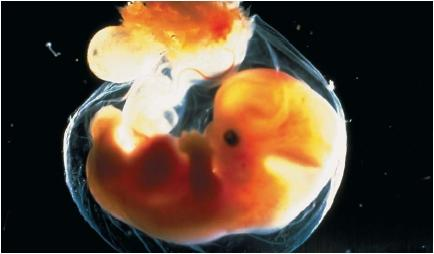
\includegraphics[width=\textwidth]{uesc_04_img0230.jpg}
  \end{center}
\end{column}
\begin{column}{.49\textwidth}
  \begin{center}
  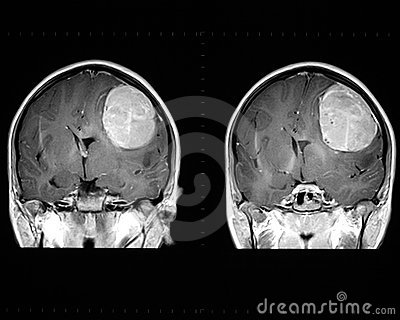
\includegraphics[width=.73\textwidth]{mri-brain-showing-tumor-1688808.jpg}
  \end{center}
\end{column}
\end{columns}

}
%%%%%%%%%%%%%%%%%%%%%%%%%%%%%
\subsection{Rakuts\"ukkel}

\frame{\frametitle{Rakuts\"ukkel}
\begin{block}{}
\begin{itemize}
\item Rakuts\"ukkel on j\"arjestikuste s\"undmuste jada mille k\"aigus rakk duplitseerib k\~{o}ik oma koostisosad ja jaguneb kaheks t\"utarrakuks.
\item Rakuts\"uklit kontrolliv 'masinav\"ark' on universaalne k\~{o}igis organismi rakut\"u\"upides.
\item Raku rakuts\"uklisse sisenemist ja 'masinav\"argi k\"aivitamist' reguleerivad raku v\"aliskeskkonna signaalid.
  \end{itemize}
\end{block}

\begin{displaymath}
\xymatrix{
                                    & \cell[blue,fill=blue]{4pt}{8pt} \\
  \cell[blue,fill=blue]{4pt}{8pt} \ar@{->}[dr] \ar@{->}[ur] &  \\
                                    & \cell[blue,fill=blue]{4pt}{8pt}  \\
}
\end{displaymath}

}
%%%%%%%%%%%%%%%%%%%%%%%%%%%%
% \subsection{Kromosomaalne ts\"ukkel}
% 
% \frame{\frametitle{Kromosomaalne ts\"ukkel}
% \begin{columns}
% \begin{column}{.55\textwidth}
% \begin{block}{2N $\rightarrow$ 4N $\rightarrow$ 2N + 2N }
% \begin{itemize}
%   \item Kromosoomide duplitseerumine ja jagunemine t\"utarrakkude vahel.
%   %\item S-faas ja M-faas on omavahel koordineeritud kuid ei kattu.
% \end{itemize}
% \end{block}
% \end{column}
% 
% \begin{column}{.44\textwidth}
% 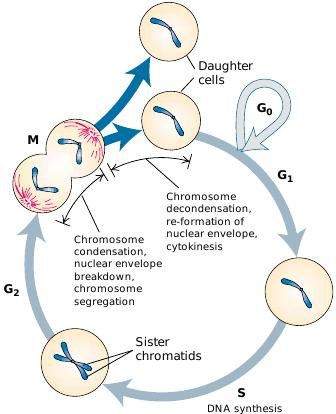
\includegraphics[width=\textwidth]{cycle1.jpg}
% \end{column}
% \end{columns}
% }
%%%%%%%%%%%%%%%%%%%%%%%%%%%%%
%%%%% Rakuts\"ukli faasid %%%%%
\section{Rakuts\"ukli faasid}
%%%%%%%%%%%%%%%%%%%%%%%%%%%%%
\subsection{Rakuts\"ukli faasid}

\frame{\frametitle{Rakuts\"ukli faasid}
\begin{columns}
\begin{column}{.5\textwidth}
\begin{block}{Neli \"uksteisele j\"argnevat faasi}
\begin{itemize}
\item G1 $\rightarrow$ S $\rightarrow$ G2 $\rightarrow$ M faas.
  \item G1, S ja G2 moodustavad \textbf{interfaasi}.
  \item Mitoosi faasid on \textbf{profaas}, \textbf{metafaas}, \textbf{anafaas} ja \textbf{telofaas}.
  \item Mittejagunev rakk on vaikeolekus (\emph{quiescence}) ehk G0 faasis.
  
\end{itemize}
\end{block}
\end{column}
\begin{column}{.5\textwidth}
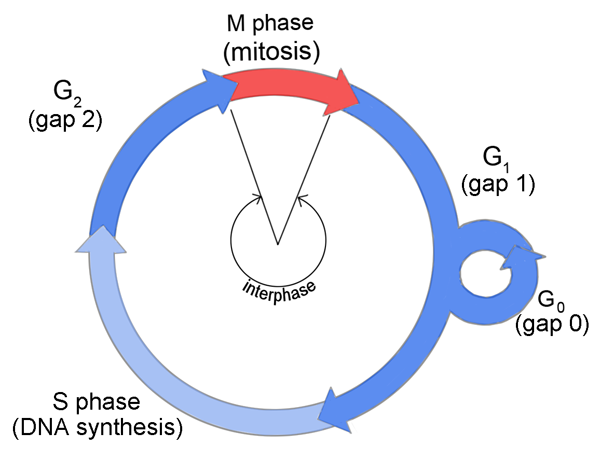
\includegraphics[width=\textwidth]{mitosis3_1}
\end{column}
\end{columns}
}
%%%%%%%%%%%%%%%%%%%%%%%%%%%
\subsection{G1-faas}
\frame{\frametitle{G$_1$-faas}

\begin{block}{}
G$_1$ on raku ts\"ukli faas, mis algab peale mitoosi ja kestab kuni DNA replikatsiooni alguseni S-faasis.
\end{block}
%\qquad
\begin{columns}
\begin{column}{.5\textwidth}
\begin{block}{G$_1$-faasis toimub}
\begin{itemize}
  \item \textbf{rakkude kasv} -- p\"armil kindlasti, imetaja rakkude puhul pole p\"aris kindel.
  \item \textbf{ettevalmistus S-faasiks} -- pre-replikatsiooni komplekside moodustumine.
\end{itemize}
\end{block}
\end{column}
\begin{column}{.5\textwidth} 
\begin{center}
\begin{figure}
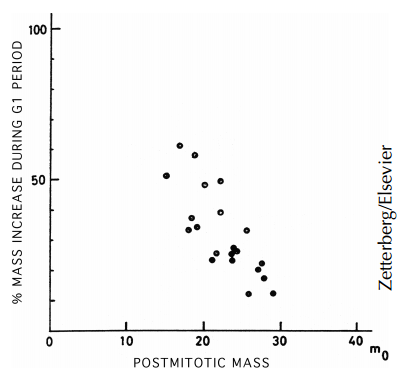
\includegraphics[width=.8\textwidth]{Zetterberg}
\caption*{\centering Rakkudel mis on G$_1$ alguses suuremad on G$_1$-s v\"aiksem juurdekasv.}
\end{figure}
\end{center}
\end{column}
\end{columns}

}
%%%%%%%%%%%%%%%%%%%%%%%%%%%%%
\subsection{S-faas}

\frame{\frametitle{S-faasis toimub genoomse DNA s\"untees}
\begin{columns}
\begin{column}{.55\textwidth}
\begin{block}{}
\begin{itemize}
  \item Kromosoomide duplitseerumine leiab aset S faasis. 
\item Kogu genoom tuleb kopeerida t\"apselt ja ainult \"uks kord. 
\item K\~oiki replikatsiooni alguspunkte kasutatakse ainult ja ainult \"uks kord.
\item Duplitseerunud \~odekromsoomid peavad j\"a\"ama k\~orvuti, mille eest vastutavad kohesiinid.
\end{itemize}
\end{block}
\end{column}

\begin{column}{.44\textwidth}
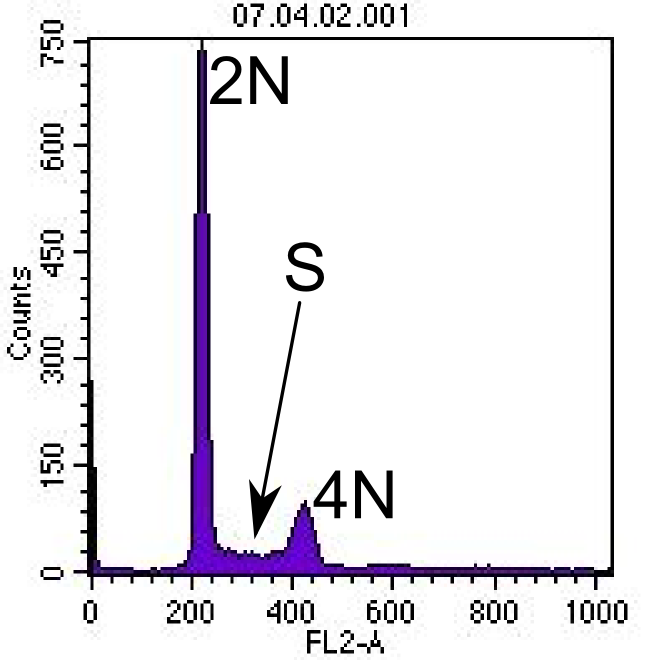
\includegraphics[width=\textwidth]{pistainingS}
\end{column}
\end{columns}
}
%%%%%%%%%%%%%%%%%%%%%%%%%%%%%
\subsection{G2-faas}
\frame{\frametitle{G$_2$-faas}
\begin{columns}
\begin{column}{.55\textwidth}
\begin{block}{G$_2$-faas on intervall DNA s\"unteesi eduka l\~opu ja mitoosis toimuva kromosoomide lahknemise vahel} 
 \begin{itemize}
  %\item 
  \item suhteliselt l\"uhike
  \item M-faasis vajalike valkude s\"untees
  \item viimane DNA kvaliteedikontroll -- G$_2$ kontrollpunkt
\end{itemize}
\end{block}
\end{column}

\begin{column}{.2\textwidth}
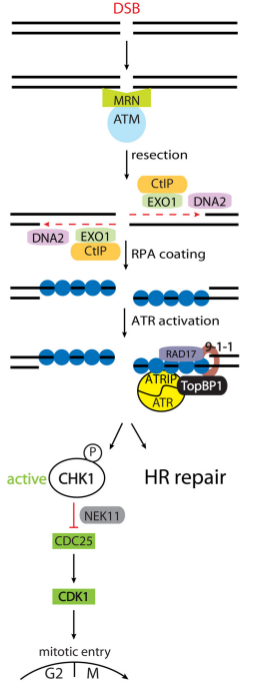
\includegraphics[width=\textwidth]{G2_check}
\end{column}
\end{columns}
 
 
}
%%%%%%%%%%%%%%%%%%%%%%%%%%%%%
\subsection{M-faas}

\frame{\frametitle{M-faasis toimub kromosoomide lahknemine}
% Profaasis toimub kromosoomide kondenseerumine v\~oimaldamaks efektiivset liikumist.
% Metafaasis joonduvad \~odekromatiidid. seostudes \"ule kinetohooride k\"a\"avi mikrotuubulitele
% Rakud peavad moodustama mitoosik\"a\"avi.
% Peale edukat k\"a\"avile seostumist vabastatakse kohesioonid ja toimub \~odekromatiidide lahknemine 
% poolustele (anafaas) kus nad dekondenseeruvad. 
\begin{columns}
\begin{column}{.6\textwidth}
\begin{block}{}
\begin{itemize}
 \item \textbf{Profaasis} toimub kromosoomide kondenseerumine.
 \item Moodustub mitoosik\"a\"av.
 \item \textbf{Metafaasis} joonduvad \~odekromatiidid.
 \item \textbf{Anafaasis} toimub \~odekromatiidide lahknemine poolustele. 
\item \textbf{Telofaasis} moodustub uuesti tuumamembraan ja tuum.
\item Ts\"utokinees.
\end{itemize}
\end{block}
\end{column}

\begin{column}{.44\textwidth}
\begin{center}
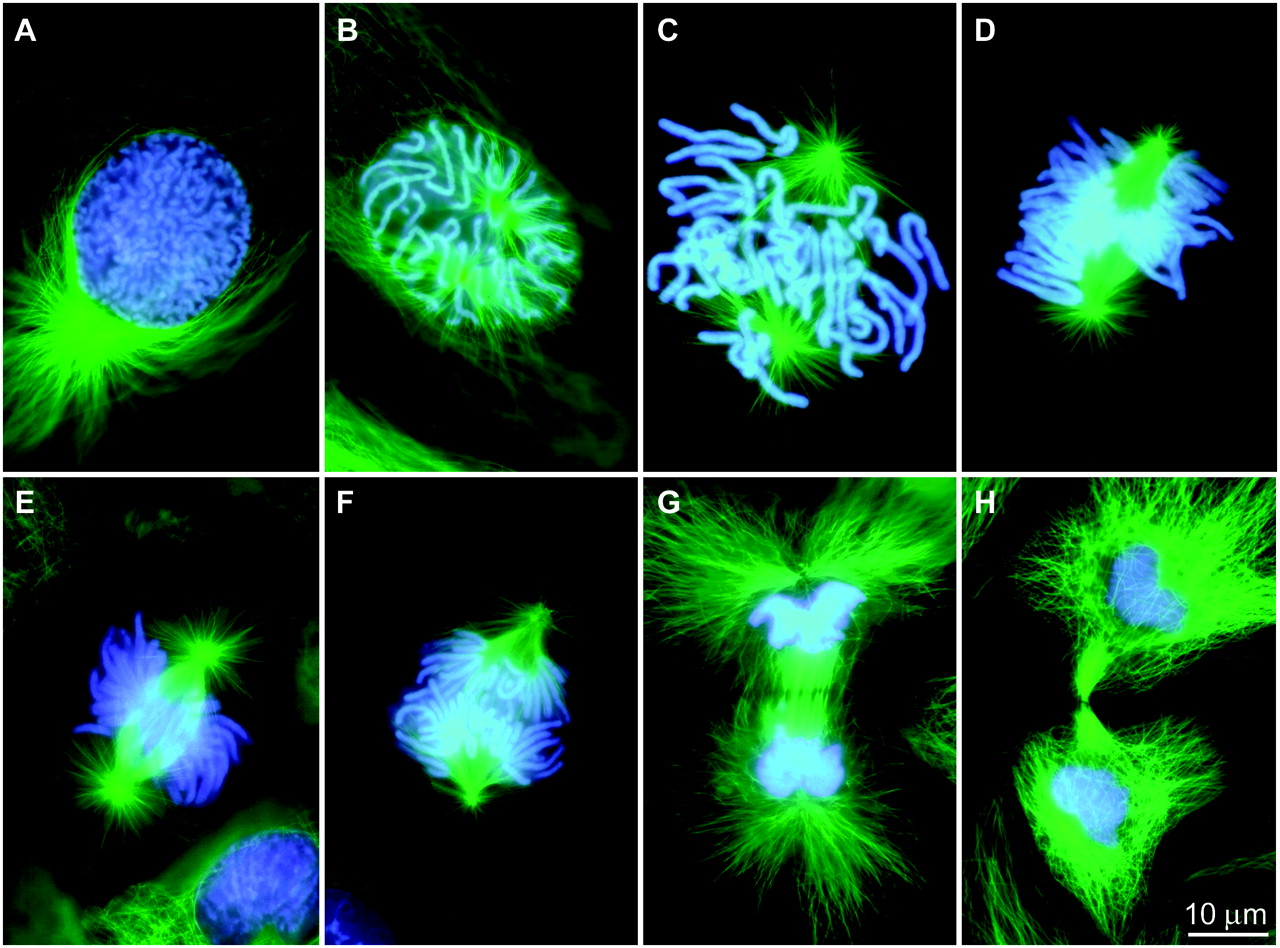
\includegraphics[width=\textwidth]{newtmitosis.jpg}
\end{center}
\end{column}
\end{columns}
}
% %%%%%%% Regulatsioon %%%%%%%%
% \section{Paradigma}
%%%%%%%%%%%%%%%%%%%%%%%%%%%%%
\subsection{Paradigma}

\frame{\frametitle{Rakuts\"ukkel liigub \"hes suunas}
\begin{block}{Kuidas tagada et rakuts\"ukli faasid toimuksid \~oiges j\"arjekorras}
\begin{itemize}  
 \item Tuuma ts\"ukli koordineerimine raku kasvu ja pooldumisega. 
 \item Replikatsioon peab toimuma vaid \"uks kord rakuts\"ukli jooksul.
 \item Replikatsioon peab eelnema kromosoomide lahknemisele.
 \item Kromosoomide lahknemine peab omakorda olema toimunud enne ts\"utokineesi e. raku jagunemist.
\end{itemize}
\end{block}
}

%%%%%%%%%%%%%%%%%%%%%%%%%%%%
\section{P\"arm}
%%%%%%%%%%%%%%%%%%%%%%%%%%%%
\subsection{P\"armigeneetika}
\frame{\frametitle{Rakkude jagunemist kontrollivate geenide kirjeldamine sai alguse p\"armis}
\begin{columns}
\begin{column}{.5\textwidth}
\begin{center}
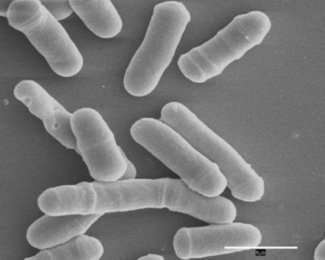
\includegraphics[width=.8\textwidth]{Fission_yeast.jpg}
\end{center}
\end{column}
\begin{column}{.5\textwidth}
\begin{block}{}
\begin{itemize}
 \item Paul Nurse jt. poolt kirjeldati poolduvas p\"armis \emph{Schizosaccharomyces pombe} mutant/geen cdc2 mis reguleerib S-faasi ja mitoosi algust.
\end{itemize}
\end{block}
\end{column}
\end{columns}
}

%%%%%%%%%%%%%%%%%%%%%%%%%%%%%
\subsection{P\"armigeneetika}
\frame{\frametitle{Temperatuuritundlike mutantide isoleerimine p\"armis}
\begin{columns}
\begin{column}{.5\textwidth}
\begin{center}
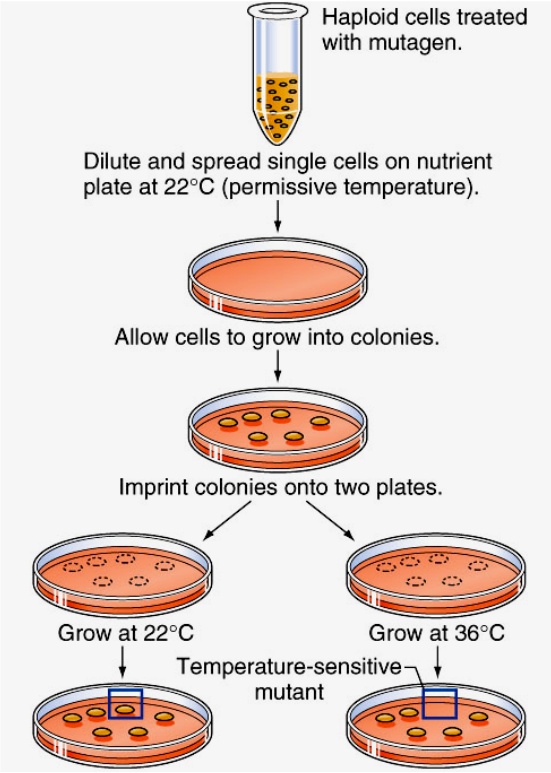
\includegraphics[width=.8\textwidth]{parmts}
\end{center}
\end{column}
\begin{column}{.5\textwidth}
\begin{block}{Haploidsetel organismidel, nagu p\"arm, on k\~oik mutatsioonid dominantsed}
\begin{itemize}
 \item Mutandid kasvavad normaalselt permissiivsel temperatuuril
 \item Mutandid kaotavad geeni funktsiooni restrikteerival temperatuuril
\end{itemize}
\end{block}
\end{column}
\end{columns}
}
%%%%%%%%%%%%%%%%%%%%%%%%%%%%
\subsection{P\"armigeneetika2}
\frame{\frametitle{P\"armi rakuts\"ukli mutandid}
\begin{columns}
\begin{column}{.5\textwidth}
\begin{center}
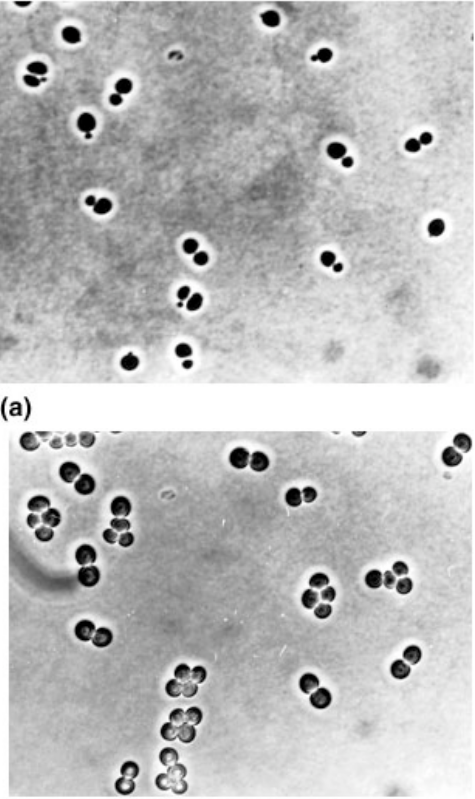
\includegraphics[width=.8\textwidth]{parmmut}
\end{center}
\end{column}
\begin{column}{.4\textwidth}
\begin{block}{}
Permissiivsel temperatuuril on p\"armipopulatsioonis erineva suurusega pungasid.
\end{block}
\vspace{1cm}
\begin{block}{}
Restrikteerival temperatuuril kasvatamine n\"aitab et rakud on l\"abinud esimese rakuts\"ukli ja arresteerunud teises.  
\end{block}
\end{column}
\end{columns}
}
%%%%%%%%%%%%%%%%%%%%%%%%%%%%%%%%%%
\subsection{P\"armumutantide seletamine}
\frame{\frametitle{Temperatuuritundlike mutantide kasutamine geeni funktsiooni sidumisel rakuts\"ukli faasiga}
\begin{center}
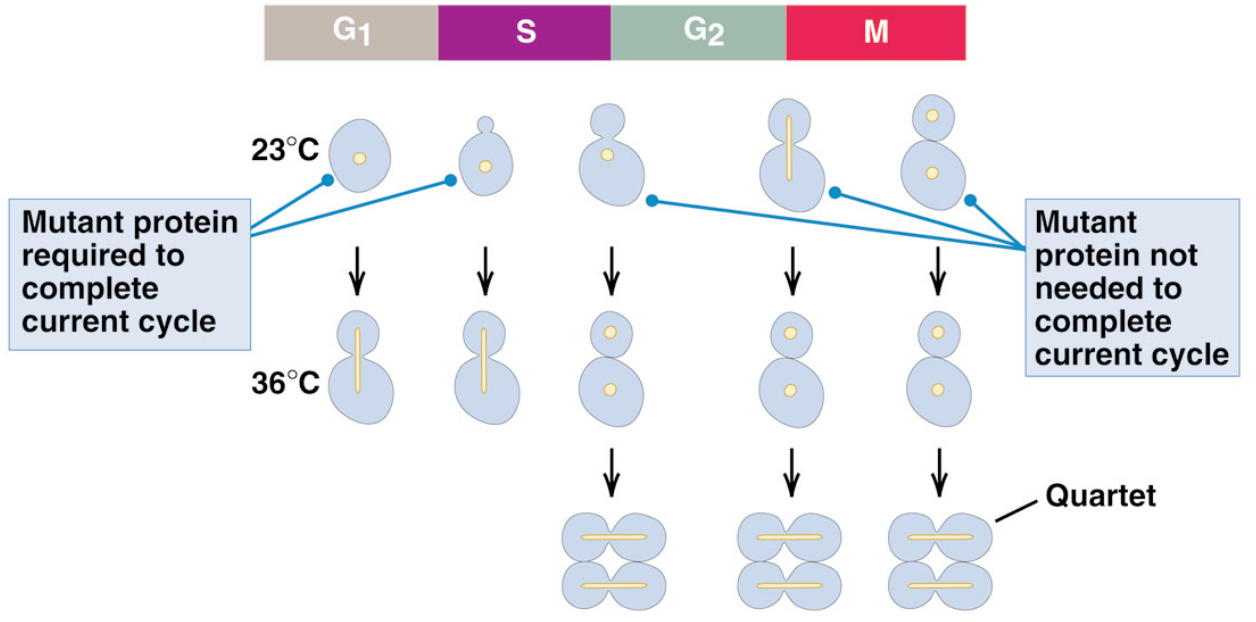
\includegraphics[width=\textwidth]{parmdeciph}
\end{center}
}
%%%%%%%%%%%%%%%%%%%%%%%%%
\subsection{Isoleerimine}
\frame{\frametitle{Mutantide isoleerimine}
\begin{center}
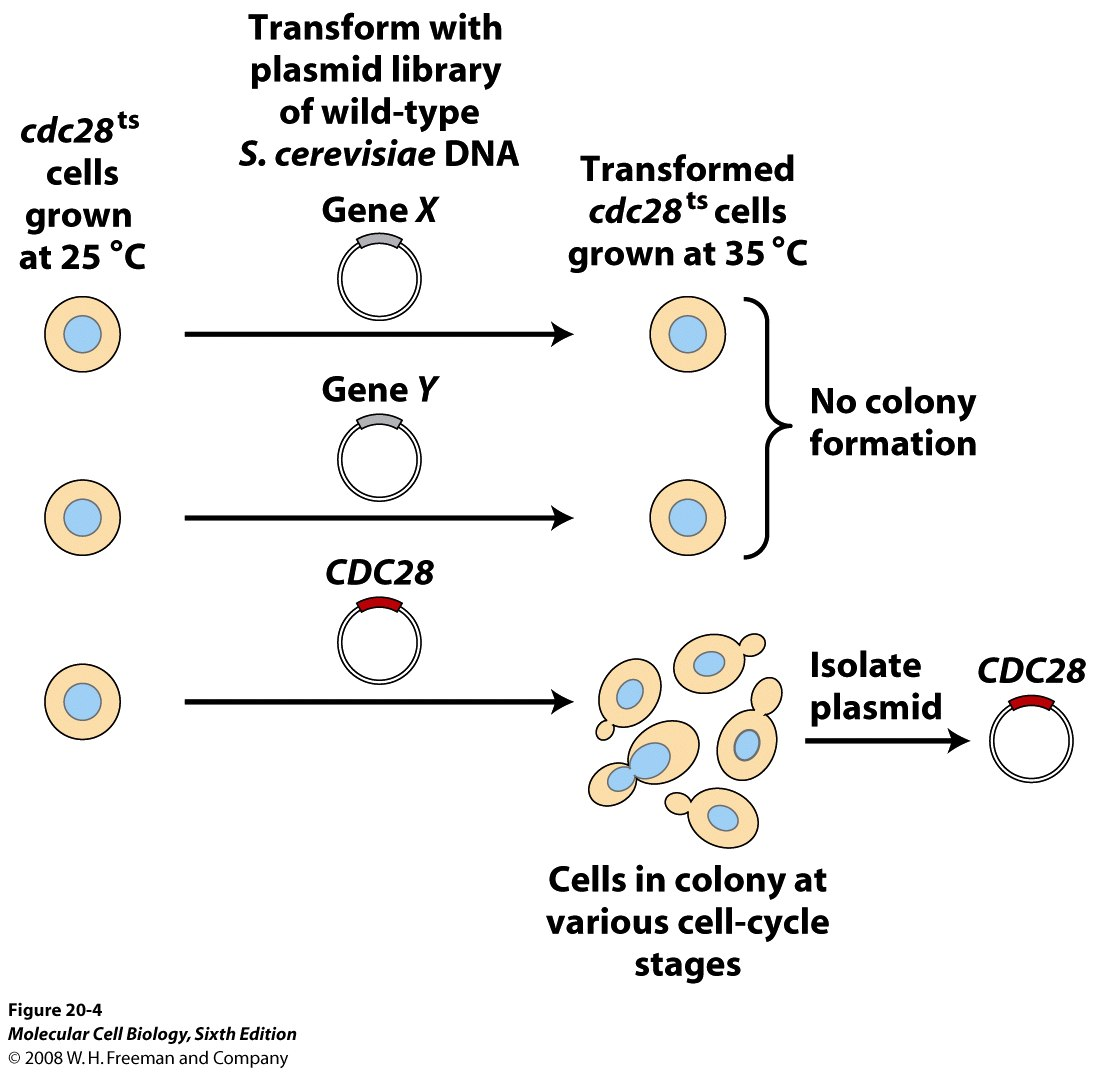
\includegraphics[width=.6\textwidth]{parmigeeniisoleerimine}
\end{center}
}

%%%%%%%%%%%%%%%%%%%%%%%%%
\subsection{P\"armigeneetika3}
\frame{\frametitle{P\"armist isoleeritud rakuts\"uklit reguleerivad geenid}
\begin{columns}
\begin{column}{.5\textwidth}
\begin{center}
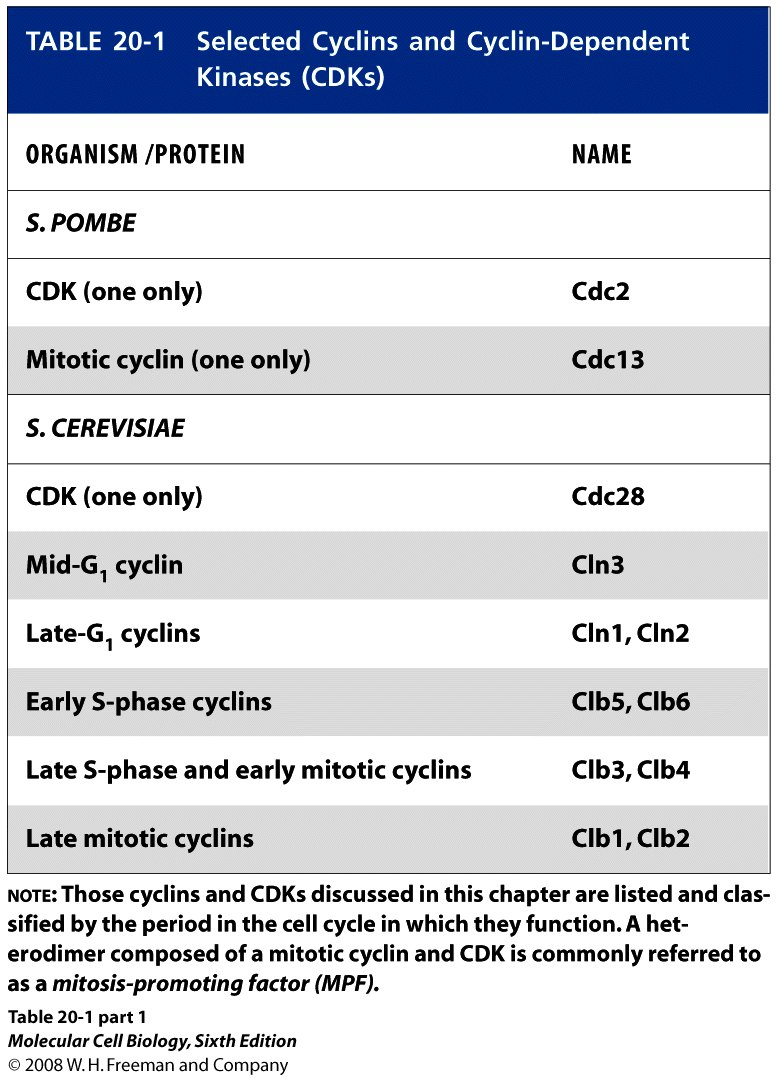
\includegraphics[width=.8\textwidth]{parmcyclins}
\end{center}
\end{column}
\begin{column}{.5\textwidth}
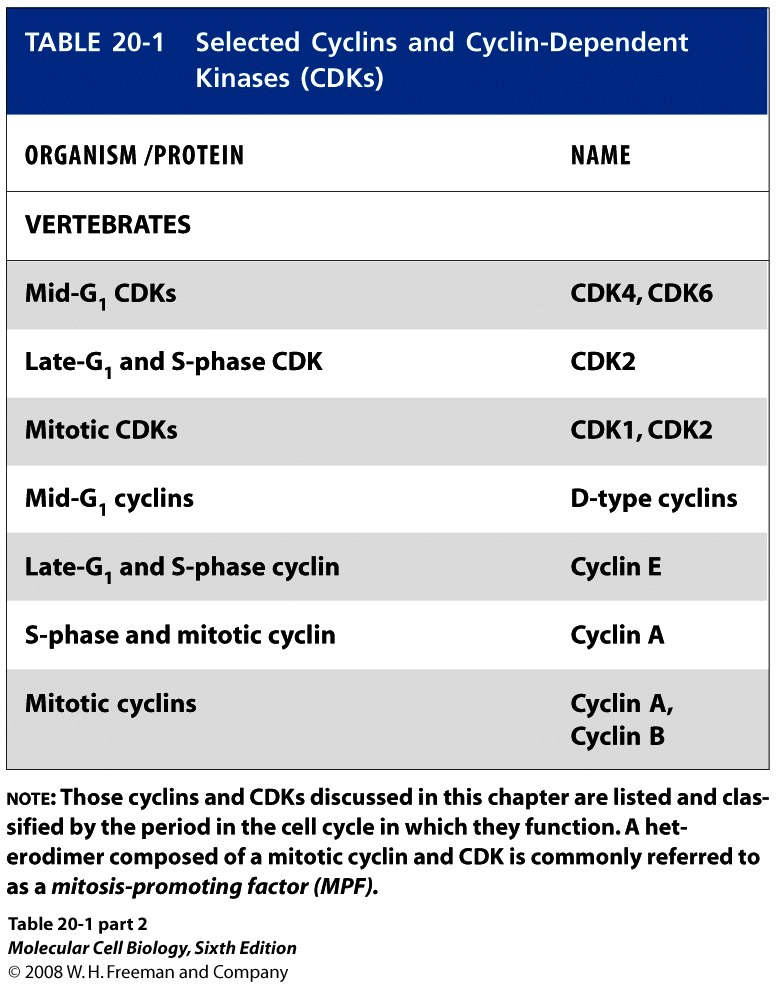
\includegraphics[width=.8\textwidth]{vertcyclins}
\end{column}
\end{columns}
}
%%%%%%%%%%%%%%%%%%%%%%%%%%%
\section{Ts\"ukliinide avastamine}
%%%%%%%%%%%%%%%%%%%%%%%%%%%%
\subsection{MPF kannuskonnas ja merisiilikus}

\frame{\frametitle{MPF kannuskonnas ja merisiilikus}
\begin{block}{}
\begin{itemize}  
 \item Aafrika kannuskonna (\emph{Xenopus laevis}) ja merisiiliku (\emph{Arbacia punctulata}) meioosi uurimine 1970 ja 1980 aastatel viis \textbf{MPF} faktori (\emph{maturation-promoting factor}) kirjeldamiseni.
\end{itemize}
\end{block}
}
%%%%%%%%%%%%%%%%%%%%%%%%%%%%%%
\subsection{Ts\"ukliinid kannuskonnas}

\frame{\frametitle{MPF kannuskonnas ja merisiilikus}
\begin{block}{1982. aastal avastasid Tim Hunt jt. merisiiliku valgus\"unteesi uurides valgud mis akumuleerusid tugevalt interfaasis ja mille tase langes kiiresti peale oots\"u\"utide jagunemist.}
\begin{itemize}   
\item Nad nimetasid need ja teised sarnaselt k\"aituvad rakuts\"uklis ostsilleeruvad valgud \textbf{ts\"ukliinideks}.
\item K\~{o}igepealt kirjeldati molekulmassist l\"ahtuvalt kaks ts\"ukliini - A ja B. 
\item Sarnasus MPF ja ts\"ukliinide vahel oli silmatorkav.
\end{itemize}
\end{block}
}

%%%%%%%%%%%%%%%%%%%%%%%%%%%
\subsection{Ts\"ukliini s\"untees on vajalik rakuts\"ukli t\"o\"os hoidmiseks}

\frame{\frametitle{Ts\"ukliini s\"untees on vajalik rakuts\"ukli t\"o\"os hoidmiseks}
\begin{block}{Marc Kirschner ja Andrew Murray uurisid 1989 ts\"ukliinide rolli Xenopuse raku ekstraktides.}
\begin{itemize}  
\item P\~{o}hinedes Yoshio Masui varasemalt l\"abi viidud t\"o\"ol, l\~{o}id nad rakuvaba mudeli mis v\~{o}is l\"abida kolm ja enam ts\"uklit.
\item Nad n\"aitasid, et valgus\"untees on vajalik \emph{in vitro} rakuts\"uklite l\"abimiseks.
\item \emph{In vitro} transkribeeritud merisiiliku ts\"ukliin B mRNA taastas rakuts\"ukli ekstraktides kus mRNA oli ens\"umaatiiselt lagundatud.
\item Samuti taastas ts\"ukli in vitro transleeritud ts\"ukliin B valk estraktides kus valgus\"untees oli blokeeritud. 

\end{itemize}
\end{block}
}
%%%%%%%%%%%%%%%%%%%%%%%%%%%%

\subsection{Ts\"ukliin B lagundamine on vajalik meioosist ja mitoosist v\"aljumisel}

\frame{\frametitle{Ts\"ukliin B lagundamine on vajalik meioosist ja mitoosist v\"aljumisel}
\begin{block}{}
\begin{itemize}  
\item Murray ja Kirschner genereerisid ts\"ukliin B amino-terminaalse deletsioonimutandi,
\begin{itemize}
  
      \item deletsioonimutant oli resistentne proteol\"u\"utilisele lagundamisele mitoosis, 
      \item kuid aktiveeris MPF-i ja viis ekstraktid M faasi. 
\end{itemize}
\item See mutant arresteeris ekstrakti M faasi. 
\item Sama juhtus ka trunkeeritud ts\"ukliini B s\"ustimisel oots\"u\"utidesse. 
\end{itemize}
\end{block}
}
%%%%%%%%%%%%%%%%%%%%%%%%%%%%
\subsection{Ts\"ukliin on otsene Cdc2 (Cdk1) regulaator}

\frame{\frametitle{Ts\"ukliin on otsene Cdc2 (Cdk1) regulaator}
\begin{block}{MPF-i puhastamine viis ts\"ukliin-kinaasi kompleksi kirjeldamiseni.}
\begin{itemize}  
\item Kuigi MPF kirjeldati juba 1971, siis puhas MPF eraldati Xenopuse munadest alles 1988.
\item Puhas MPF sisaldas kahte valku massiga 32 kDa ja 45 kDa ning omas kinaasset aktiivsust (Lohka et al., 1988). 32 kDa valk v\~{o}is olla Cdc2.
\item P\"armi Cdc2 konserveerunud 16-aa j\"arjestuse vastane antikeha (nn. PSTAIRE antikeha) sadestas MPF-ist kinaasse aktiivsuse massiga 32 kDa ( Gautier et al., 1988).
\item Puhas Cdc2 \"uksi ei n\"aidanud kinaasset aktiivsust.
\item L\~{o}puks n\"aidatigi, et merekarbi (\emph{Spisula solidissima}) embr\"uote homogenaadist ko-sadestusid ts\"ukliinid koos Cdc2 kinaasse aktiivsusega (Draetta et al., 1989).
\end{itemize}
\end{block}
}
%%%%%%%%%%%%%%%%%%%%%%%%%%%%%
\subsection{Kirjeldati uus klass kinaase}
\frame{\frametitle{Kirjeldati uus klass kinaase}
\begin{columns}
\begin{column}{.5\textwidth}
\begin{center}
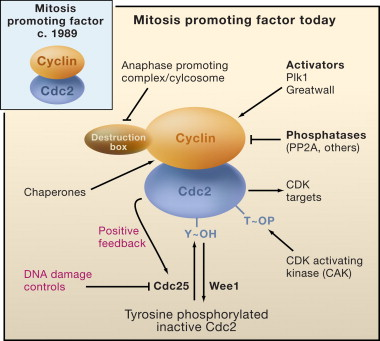
\includegraphics[width=.8\textwidth]{cdc2mpf.jpg}
\end{center}
\end{column}
\begin{column}{.5\textwidth}
\begin{block}{}
\begin{itemize}
 \item K\~{o}ik ts\"ukliinidega seotud kinaasid otsustati 1991. aastal nimetada ts\"ukliin-s\~{o}ltuvateks kinaaasideks ehk \emph{i.k.} \textbf{CDK}. 
  \item Cdc2 nimetati nii esimesena Cdk1.
\end{itemize}
\end{block}
\end{column}
\end{columns}
}

%%%%%%%%%%%%%%%%%%%%%%%%%%%%
\section{Regulatsioon}
%%%%%%%%%%%%%%%%%%%%%%%%%%%%
\subsection{ts\"ukliin-CDK kompleksi j\"arjestikune aktivatsioon}

\frame{\frametitle{Ts\"ukliin-CDK komplekside j\"arjestikune aktivatsioon}
\begin{center}
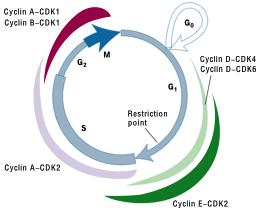
\includegraphics[width=.4\textwidth]{cyclinsincellcycle}
\vspace{0.5cm}
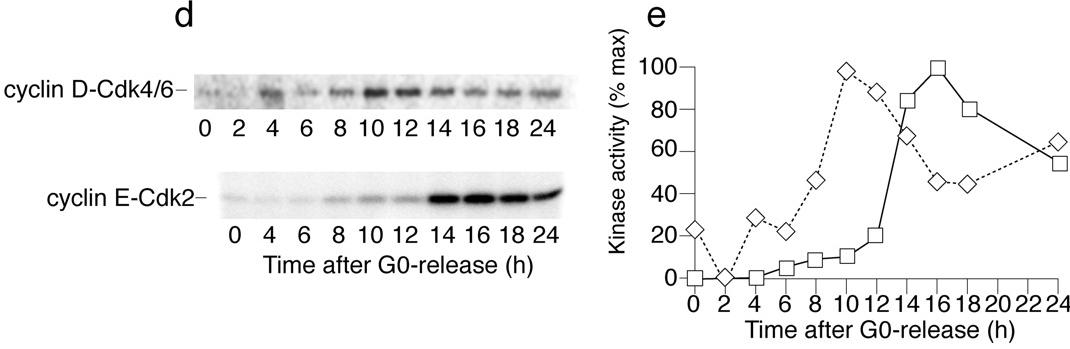
\includegraphics[width=.7\textwidth]{cyclinsincellcycleAnnica}
\end{center}
}

%%%%%%%%%%%%%%%%%%%%%%%%%%%%%
\subsection{Ts\"ukliinid}

\frame{\frametitle{Ts\"ukliinid ja ts\"ukliin kinaasid}
\begin{block}{}
Ts\"ukliin-s\~oltuvad kinaasid (CDK) reguleerivad rakuts\"uklit fosfor\"uleerides teisi valke 
\end{block}
\begin{center}
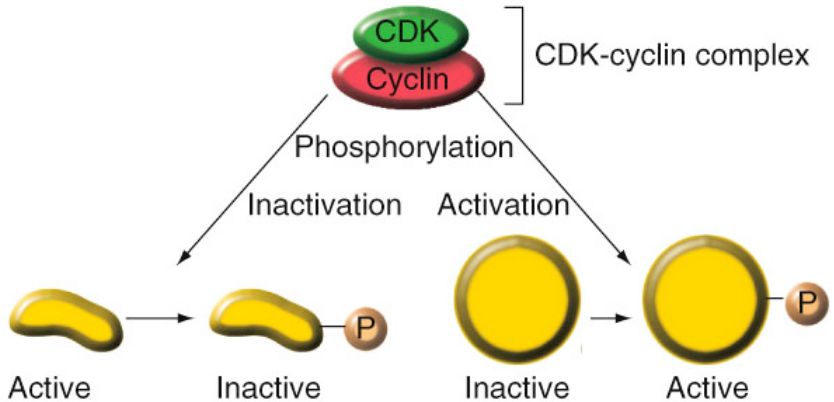
\includegraphics[width=.7\textwidth]{cdkscontrolcycle}
\end{center}
}
%%%%%%%%%%%%%%%%%%%%%%%%%%%%%
\subsection{Ts\"ukliini substraat}

\frame{\frametitle{Ka rakuts\"ukli masinav\"arki reguleerivad kinaasid}
\begin{columns}
\begin{column}{.6\textwidth}
\begin{block}{CDK substraadid}
\begin{itemize}
  \item Tsentrosoomi valke (CP110) fosfor\"uleeritakse G1/S \"uleminekul tsentrosoomi duplitseerumiseks.
  \item Enne S-faasi aktiveeritakse replikatsioonikompleks (Treslin).
  \item Histoonide fosfor\"uleerimine S ja M faasis kromatiini kondenseerumiseks.
\item Tuumamebraani valkude (Lamiin) fosor\"uleerimine p\~{o}hjustab tuumamembraani lagunemise M-faasis.
\end{itemize}
\end{block}
\end{column}
\begin{column}{.4\textwidth}
\begin{center}
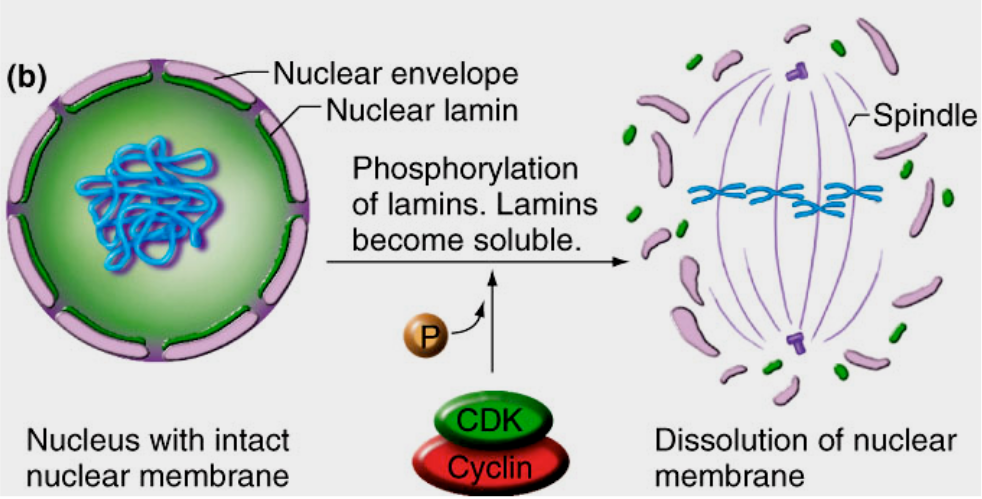
\includegraphics[width=\textwidth]{lamiinidoncdksubstraat}
\end{center}
\end{column}
\end{columns}
}

%%%%%%%%%%%%%%%%%%%%%%%%%%%%%
\subsection{Ts\"ukliinid}

\frame{\frametitle{Rakuts\"ukli eri faasides on aktiivsed erinevad ts\"ukliin-kinaasi kompleksid}
\begin{center}
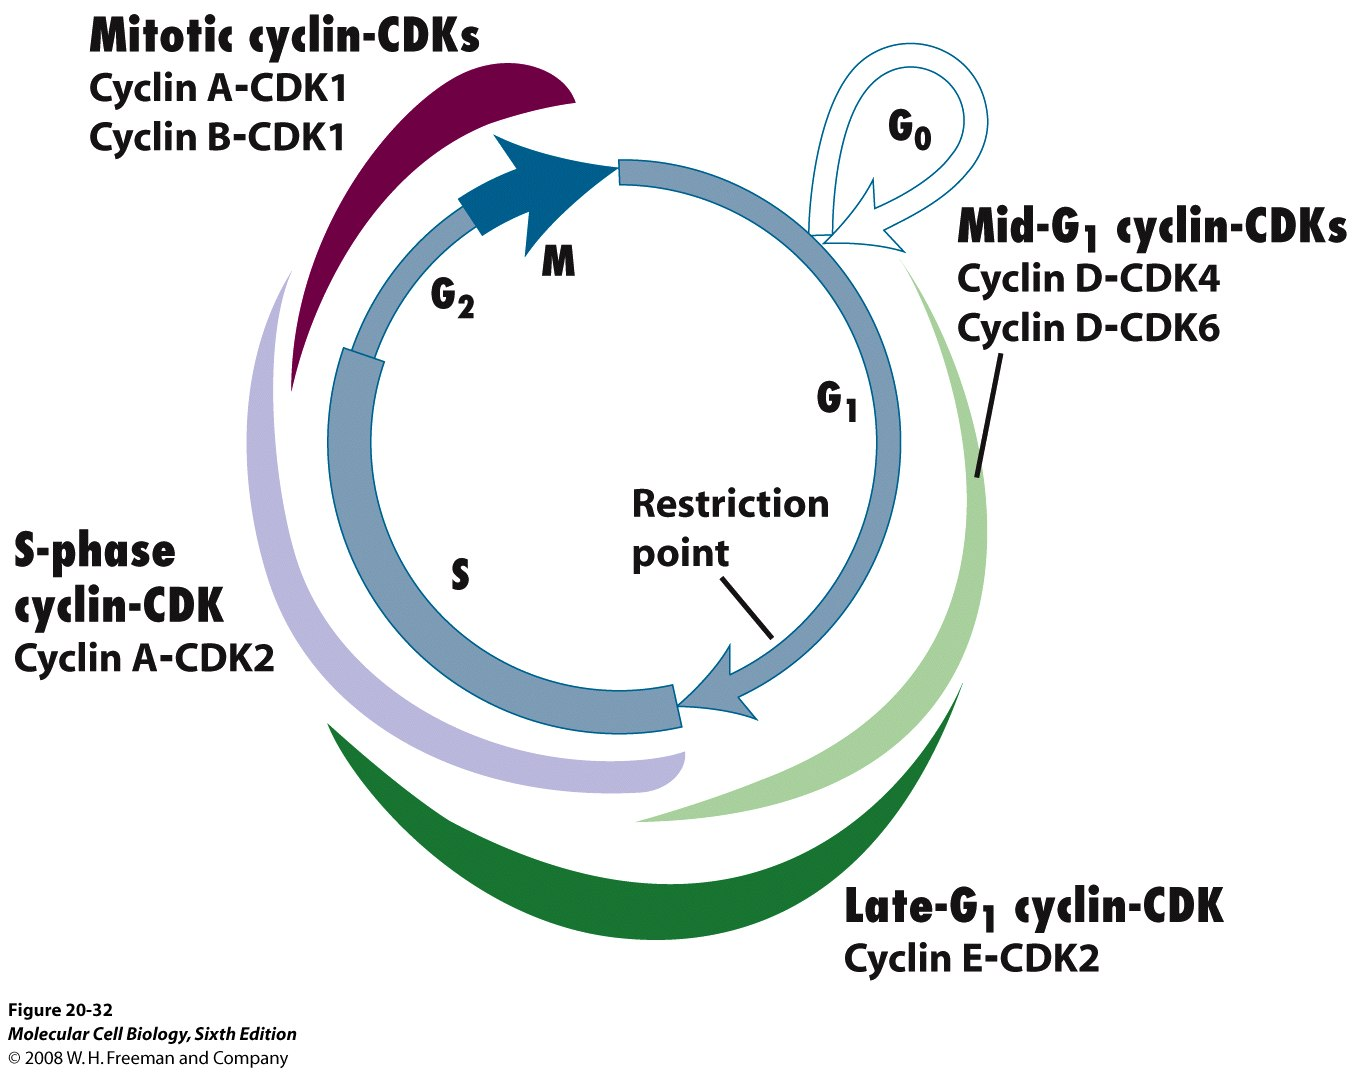
\includegraphics[width=.8\textwidth]{tsykliinid}
\end{center}
}
%%%%%%%%%%%%%%%%%%%%%%%%%%%%
\subsection{Ts\"ukliinide tase muutub}

\frame{\frametitle{Ts\"ukliinide hulk rakus muutub rakuts\"ukli k\"aigus}

\begin{itemize}
  \item Ts\"ukliine kontrollitakse l\"abi proteol\"u\"utilise lagundamise.
\item Ts\"ukliini j\"arkj\"arguline t\~{o}us ja kiire lagundamine tagab rakuts\"ukli 'hammasrataste' liikumise \"uhes sunas.
\item D-ts\"ukliinid erinevad: nende puhu ei toimu j\"arske k\~{o}ikumisi rakuts\"ukli k\"aigus.
\item D-ts\"ukliinid on reguleeritud mitogeensete sinaalide poolt.
\end{itemize}
\begin{center}
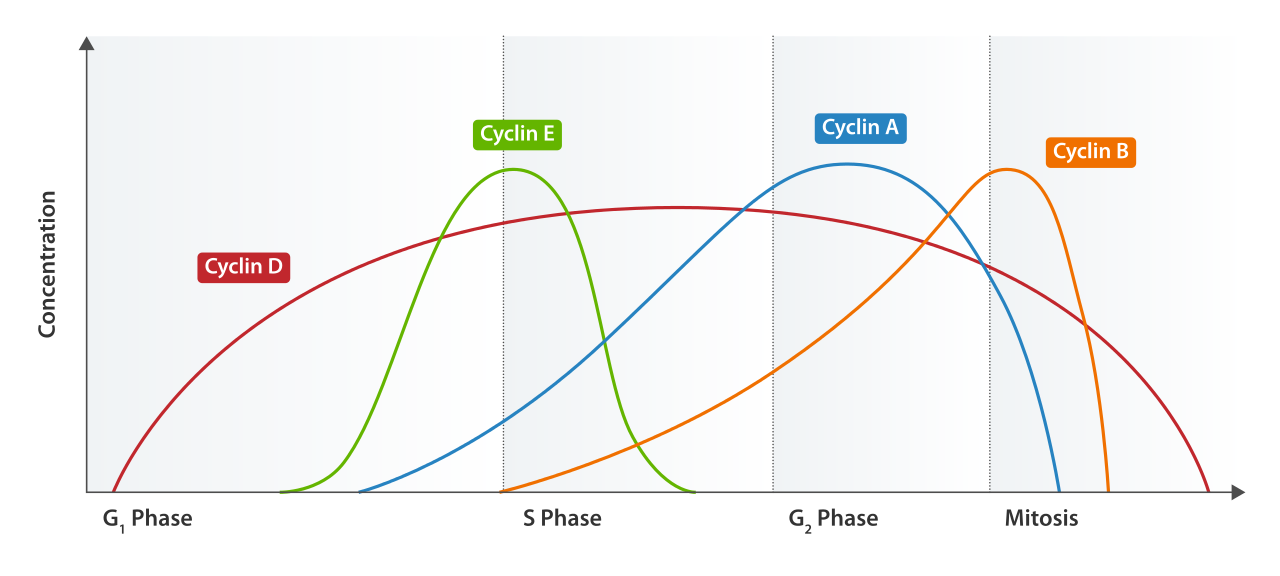
\includegraphics[width=.8\textwidth]{CyclinExpression}
\end{center}
}
%%%%%%%%%%%%%%%%%%%%%%%%%%%%
\subsection{CDKI}

\frame{\frametitle{Lisaks ts\"ukliinidele reguleerivad ts\"ukliin-s\~{o}ltuvaid kinaase ka CDK inhibiitorid (CdkI)}
Praeguseks on kirjeldatud seitse erinevat CdkI-d.
\begin{itemize}
  \item INK4 valgud (\textbf{in}hibitors of CD\textbf{K4}), mis inhibeerivad spetsiifiiselt ainult CDK4 ja CDK6.
  \begin{itemize}
  \item p16$^{INK4A}$, p15$^{INK4B}$, p18$^{INK4C}$, p19$^{INK4D}$.
\end{itemize}
\item p21$^{Cip1}$ , p27$^{Kip1}$ , p57$^{Kip2}$ : inhibeerivad k\~{o}iki teisi ts\"ukliin-CDK komplekse.

\end{itemize}
\begin{center}
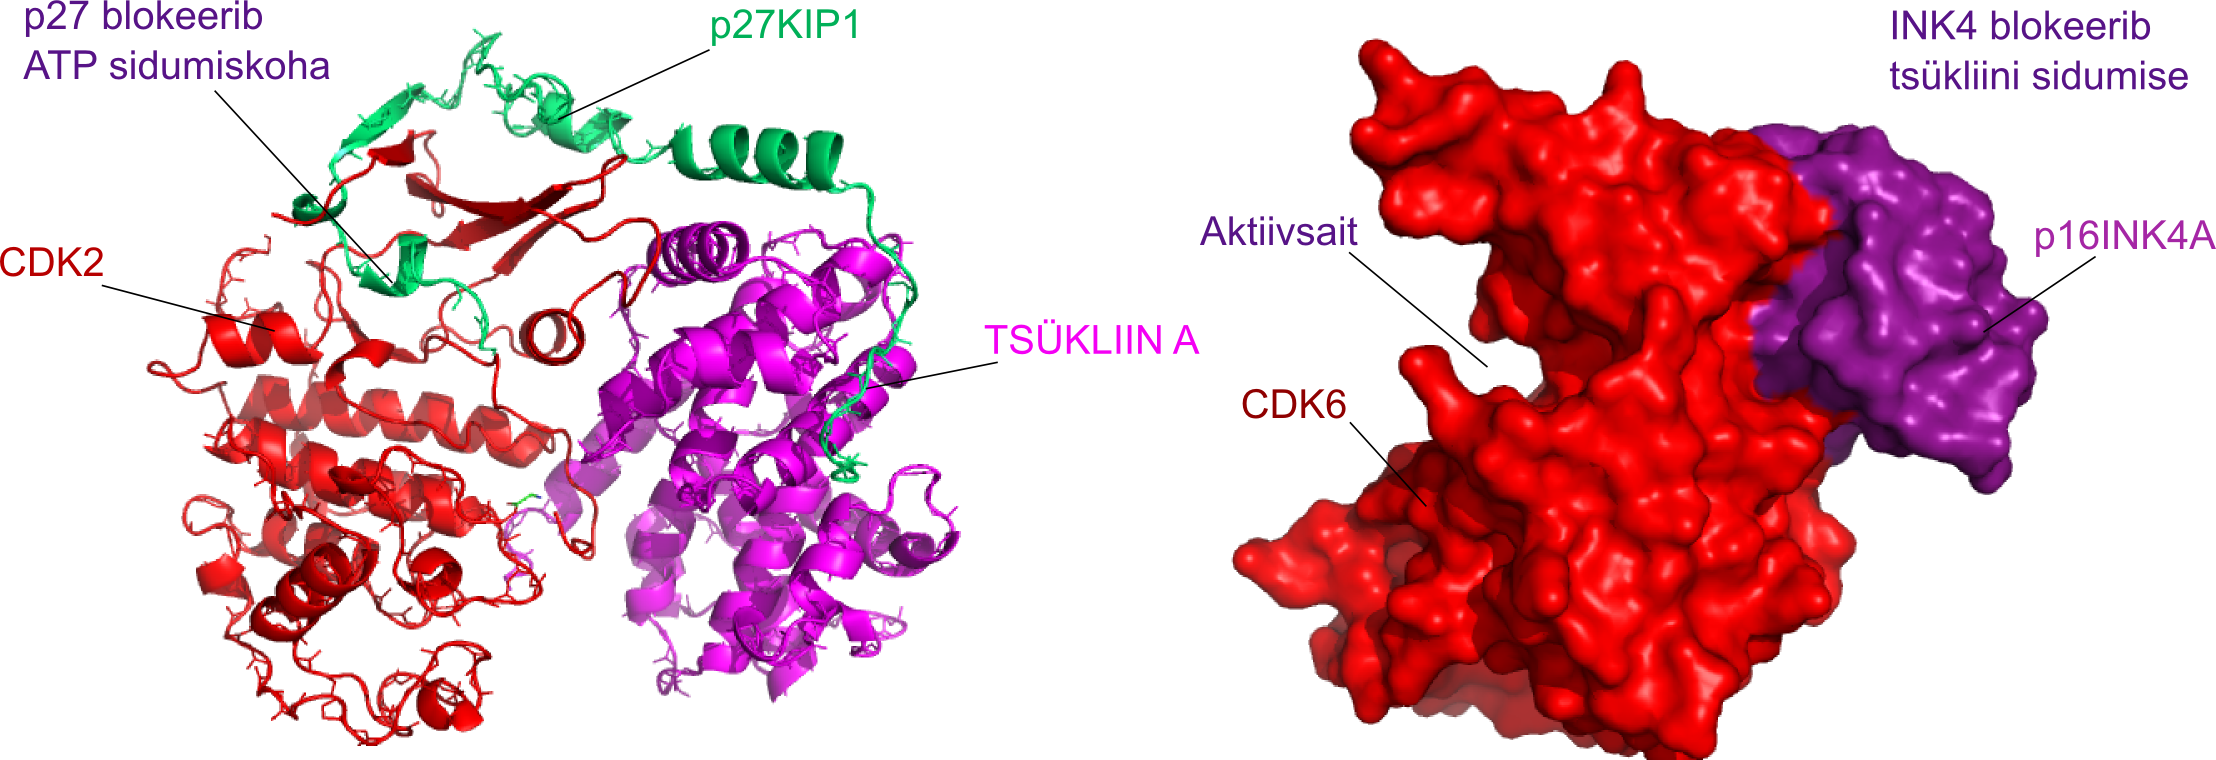
\includegraphics[width=.8\textwidth]{p16-p27mech}
\end{center}
}
%%%%%%%%%%%%%%%%%%%%%%%%%%%%%
\subsection{INK4B}

\frame{\frametitle{TGF-$\beta$ indutseerib p15$^{INK4B}$}

\begin{itemize}
  \item TGF-$\beta$ peamine raku jagunemist pidurdav mehhanism t\"o\"otab l\"abi p15$^{INK4B}$.
\item p15$^{INK4B}$ blokeerib ts\"ukliin D-CDK4/6 komplekside moodustumise ja inhibeerib olemasolevaid.
\item Ilma aktiivse ts\"ukliin D-CDK4/6 pole rakuts\"ukkel v\~{o}imeline arenema l\"abi varase ja keskmise G1 faasi restriktsioonipunktini.
\item Kui rakk on juba restriktsioonipunkti l\"abinud pole enam D-CDK4/6 aktiivsus vajalik.
\item Peale restriktsioonipunkti muutub rakk 'tundetuks' ka TGF-$\beta$ inhibeerivale toimele.
\end{itemize}
}
%%%%%%%%%%%%%%%%%%%%%%%%%%%%%
\subsection{p21}
\frame{\frametitle{p21Cip1 aktiveeritakse vastusena stressile}

\begin{itemize}
  \item p21Cip1 toimib l\"abi terve rakuts\"ukli.
\item Peamine p21Cip1 induktor on DNA kahjustused.
\item p21Cip1 inhibeerib E-CDK2, A-CDK2, A-CDC2, B-CDC2 komplekse.
\item Kui DNA kahjustused on parandatud, siis v\~{o}etakse p21Cip1-blokk maha.
\end{itemize}
}
%%%%%%%%%%%%%%%%%%%%%%%%%%%%%
%%%%%%% Kontrollid %%%%%%%%%%
\section{Kontrollid}
\subsection{Kontrollid}
\frame{\frametitle{Rakuts\"ukli kontrollpunktid}
\begin{block}{Genoomi stabiilsuse rakuts\"uklis tagavad \emph{checkpointid}}
\begin{itemize}
  \item \textbf{G1-S DNA kahjustuste kontrollpunkt}: S-faasi sisenemine on blokeeritud kui genoom on vigane.
 \item \textbf{S-faasi kontroll}: replikatsioon aeglustub v\~{o}i seiskub vastusena DNA kahjustustele.
 \item \textbf{G2-M kontroll} blokeerib raku mitoosi sisenemise kuni genoomi replikatsioon S-faasis on l\~{o}pule viidud.
 \item \textbf{M faasis kontrollpunkt} mis blokeerib sisenemise anafaasi kuni k\~{o}ik kromosoomid on korrektselt k\"a\"avile kinnitunud.
 \item Eksisteerib veel \textbf{hilise G2 dekatenatsiooni kontroll} mis monitoorib, et kromosoomid ei oleks omavahel 's\~{o}lmes'.
\end{itemize}
\end{block}
}
%%%%%%%%%%%%%%%%%%%%%%%%%
\subsection{Rad17}

\frame{\frametitle{Rad17: genoomi replitseeritakse ainult \"uks kord}
Rad17 sensorvalgu fosfr\"uleerimine ATRi poolt on vajalik DNA-kahjustuste poolt indutseeriud G2-faasi blokiks.
\begin{columns}
\begin{column}{.6\textwidth}
\begin{block}{Komosoomi aberratioonid RAD17 flox/- rakkudes. }
\begin{itemize}
  \item Katkenud komosoomid (all vasak, nool).
  \item Endoreduplitseerunud kromosoomid (all parem).
  \end{itemize}
\end{block}
\end{column}
\begin{column}{.4\textwidth}
\begin{center}
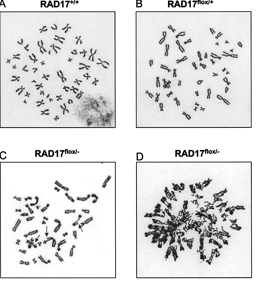
\includegraphics[width=\textwidth]{Rad17}
\end{center}
\end{column}
\end{columns}
}
%%%%%%%%%%%%%%%%%%%%%%%%%
\subsection{ATR}

\frame{\frametitle{ATR replikatsiooni \emph{check}}
Seriin-treoniin kinaas ATR tagab fragiilsete saitide stabiilsuse.
\begin{columns}
\begin{column}{.5\textwidth}
\begin{center}
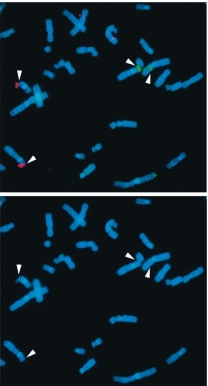
\includegraphics[width=.6\textwidth]{ATR}
\end{center}
\end{column}
\begin{column}{.5\textwidth}
\begin{block}{}
\begin{itemize}
  \item \textbf{ATR aktiveeritakse vastuseks \"uheahelalisele DNA-le}.
  \item Aktiveeritud ATR fosfor\"uleerib CHK1 kinaasi ja k\"aivitatakse signaalirada mis viib rakuts\"ukli blokini.
  \end{itemize}
\end{block}
\end{column}
\end{columns}
}

%%%%%%%%%%%%%%%%%%%%%%%%%%%
\subsection{BUB}

\frame{\frametitle{BUB1: k\"a\"avi kontrollpunkt}
K\"a\"avi kontrollpunkt (\emph{spindle assembly checkpoint, SAC}) hoiab \"ara aneuploidia tekke.
\begin{columns}
\begin{column}{.6\textwidth}
\begin{block}{}
\begin{itemize}
  \item Mutatsioonid mitoosik\"a\"avi kontrollpunktis v\~{o}ib p\~{o}hjustada kromosomaalse ebastabiilsuse ja aneuploidsuse, 
  \item \"ule 90\% tahketest kasvajatest sisaldab kromosomaalseid aberratsioone.
  \item BUB1 funktsiooni eksperimentaalne p\"arssimine on piisav rakkudes aneuploidse fenot\"u\"upi tekkeks.
  \end{itemize}
\end{block}
\end{column}
\begin{column}{.4\textwidth}
See BUB1-vaigistatud rakk on kaotanud kromosoomid 1 ja 6. 
\begin{center}
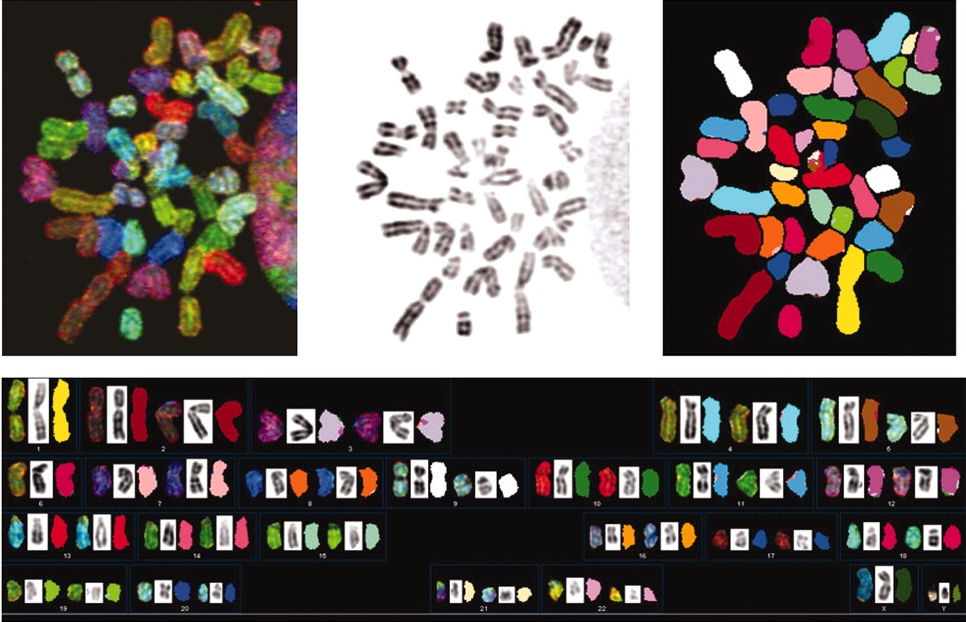
\includegraphics[width=\textwidth]{BUB}
\end{center}
\end{column}
\end{columns}
}
%%%%%%%%%%%%%%%%%%%%%%%%%
\subsection{Restriktsioon}

\frame{\frametitle{G$_1$ restriktsioonipunkt}

\begin{block}{Tagab mitogeense kontrolli rakuts\"ukli kulgemise \"ule.}
\begin{itemize}
  \item Varases- ja keskmises G1 faasis on S-faasi sisenemine seerum s\~{o}ltuv.
  \item Samuti on rakud tundlikud TGF-$\beta$ anti-mitogeensele toimele.
  \item Hilises G1 faasis on rakud juba p\"uhendunud S-faasi sisenemisele ja ei s\~{o}ltu enam rakuv\"alistest signaalidest.
\end{itemize}
\end{block}

}
%%%%%%%%%%%%%%%%%%%%%%%
\subsection{R-point}

\frame{\frametitle{RB fosfor\"ulatsioon reguleerib restriktsioonipunkti}

\begin{itemize}
  \item Kui rakud l\"abivad M/G1 \"ulemineku, siis RB defosfor\"uleeritakse t\"aielikult.
  \item G1 faasis ts\"ukliin D-CDK4/6 h\"upofosfor\"uleerib RB.
  \item H\"upofosfor\"uleeritud RB muutub ts\"ukliin E-CDK2 substraadiks ja h\"uperfosfor\"uleeritakse.
 \item RB j\"a\"ab h\"uperfosfor\"uleerituks kogu \"ulej\"a\"anud raku ts\"ukli (kuni j\"alle G1-ni).
  \end{itemize}
  \begin{center}
  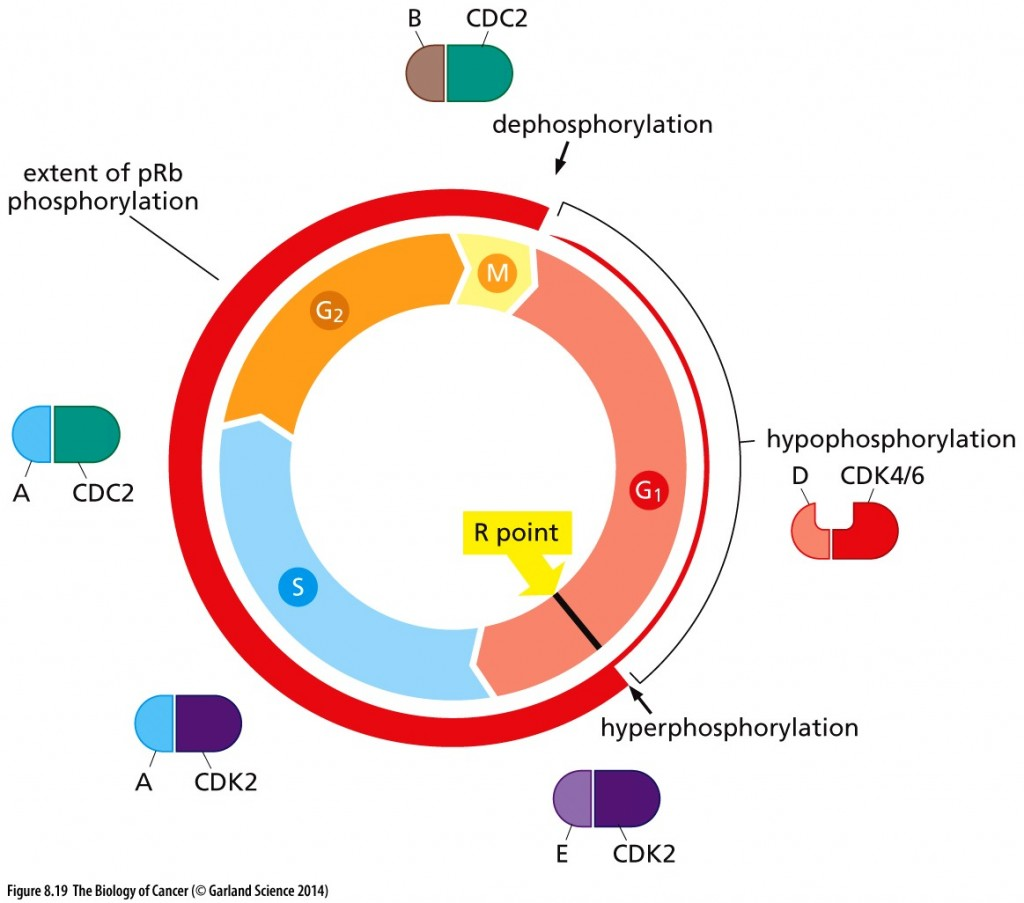
\includegraphics[width=.4\textwidth]{restrictionpoint.jpg}
\end{center}
}

%%%%%%%%%%%%%%%%%%%%%%%%
\subsection{G1Skontroll}
\frame{\frametitle{G$_1$$\rightarrow$S kontroll: raku kasv ja rakuv\"alised signaalid}

\begin{center}
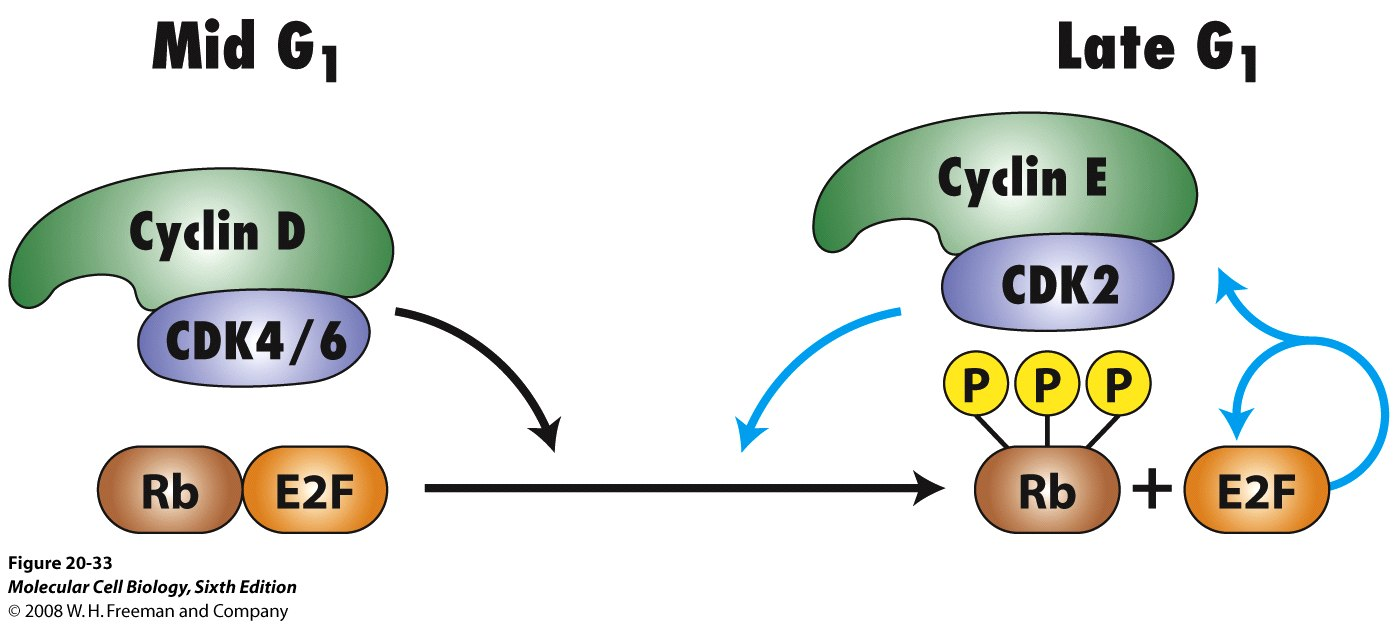
\includegraphics[width=.8\textwidth]{g1scheck}
\end{center}

\begin{columns}
\begin{column}{.49\textwidth}
\begin{block}{Positiivsed signaalid}
\begin{itemize}
  \item kasv, elluj\"a\"amissignaalid, mitogeenid
\end{itemize}
\end{block}
\end{column}
\begin{column}{.49\textwidth}
\begin{block}{Negatiivsed signaalid}
\begin{itemize}
  \item ts\"utostaatilised, genotoksilised, metaboolsed, 
  onkogeensed, oks\"udatiivne stress
\end{itemize}
\end{block}
\end{column}
\end{columns}
}
%%%%%%%%%%%%%%%%%%%%%%%%%%%%%%
\subsection{E2F}

\frame{\frametitle{E2F m\"arklaudgeenid}
\begin{columns}
\begin{column}{.5\textwidth}
\begin{block}{}
\begin{itemize}
  \item \textbf{ts\"ukliin E},
  \item \textbf{DNA replikatsiooni toetava kompleksi valgud}: ORC-id, MCMs, DNA polymerase alfa,
  \item \textbf{j\"argmistes sammudes vajalikud valgud}: ts\"ukliin B, Cdk1 ja erinevad DNA kvaliteedikontrolli valgud.
\end{itemize}
\end{block}
\end{column}
\begin{column}{.5\textwidth}
\begin{center}
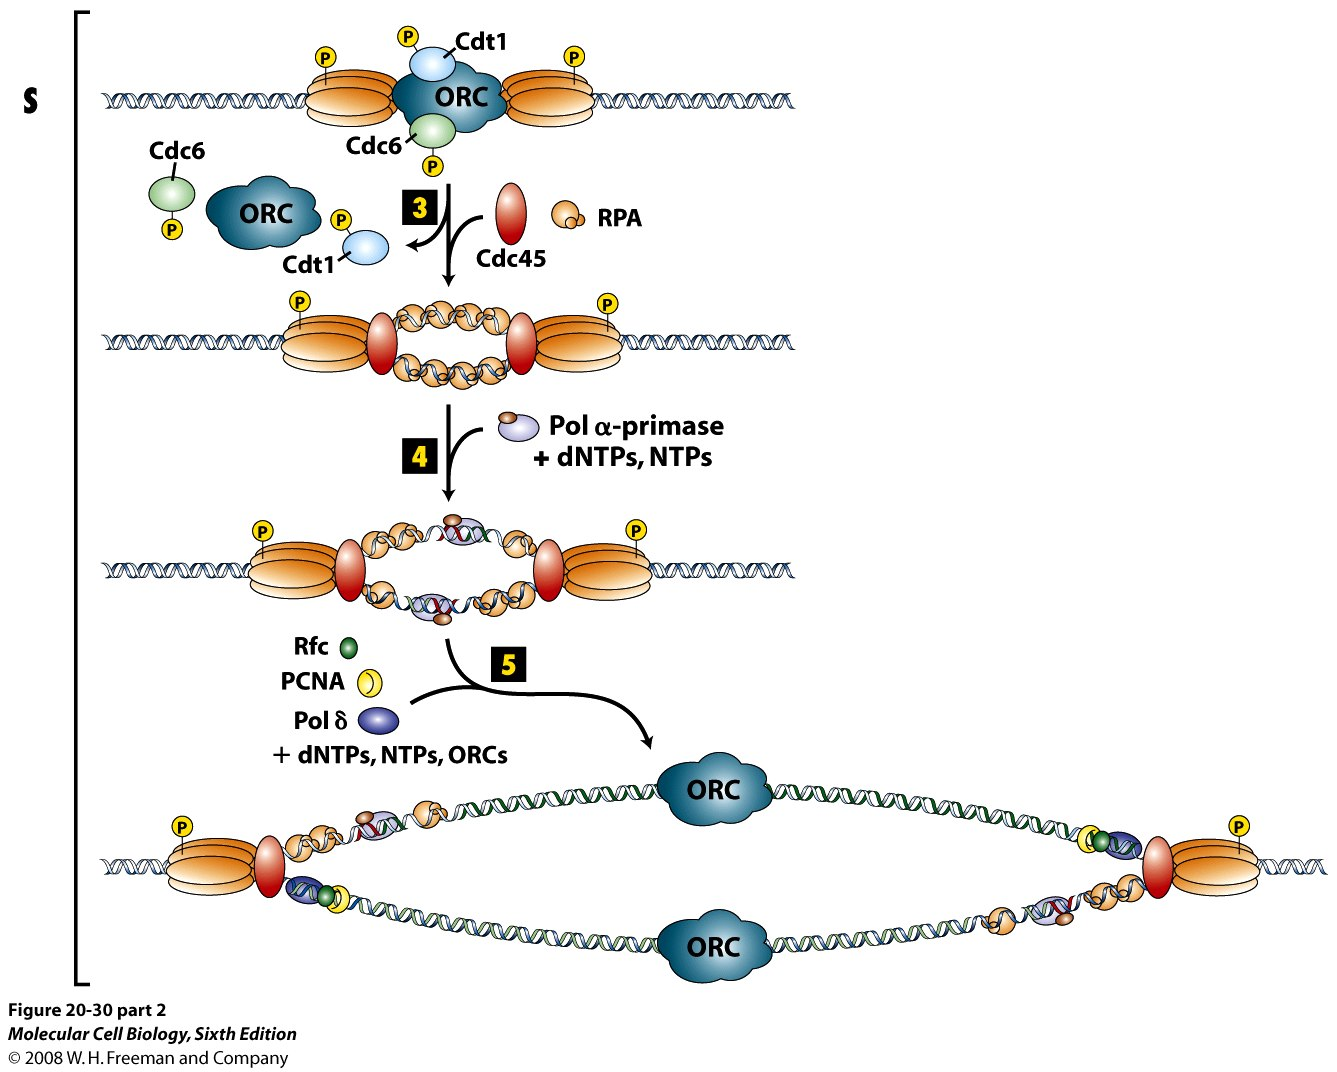
\includegraphics[width=\textwidth]{sproteins}
\end{center}
\end{column}
\end{columns}
}
%%%%%%%%%%%%%%%%%%%%%%%%%%%%%%
% DNA metabolismi checkpoint %
\subsection{DNAkontroll}
\frame{\frametitle{DNA metabolismi kontroll: ATM \& ATR -- DNA kahjustusi kontrollivad kinaasid}

\begin{columns}
\begin{column}{.6\textwidth}
\begin{center}
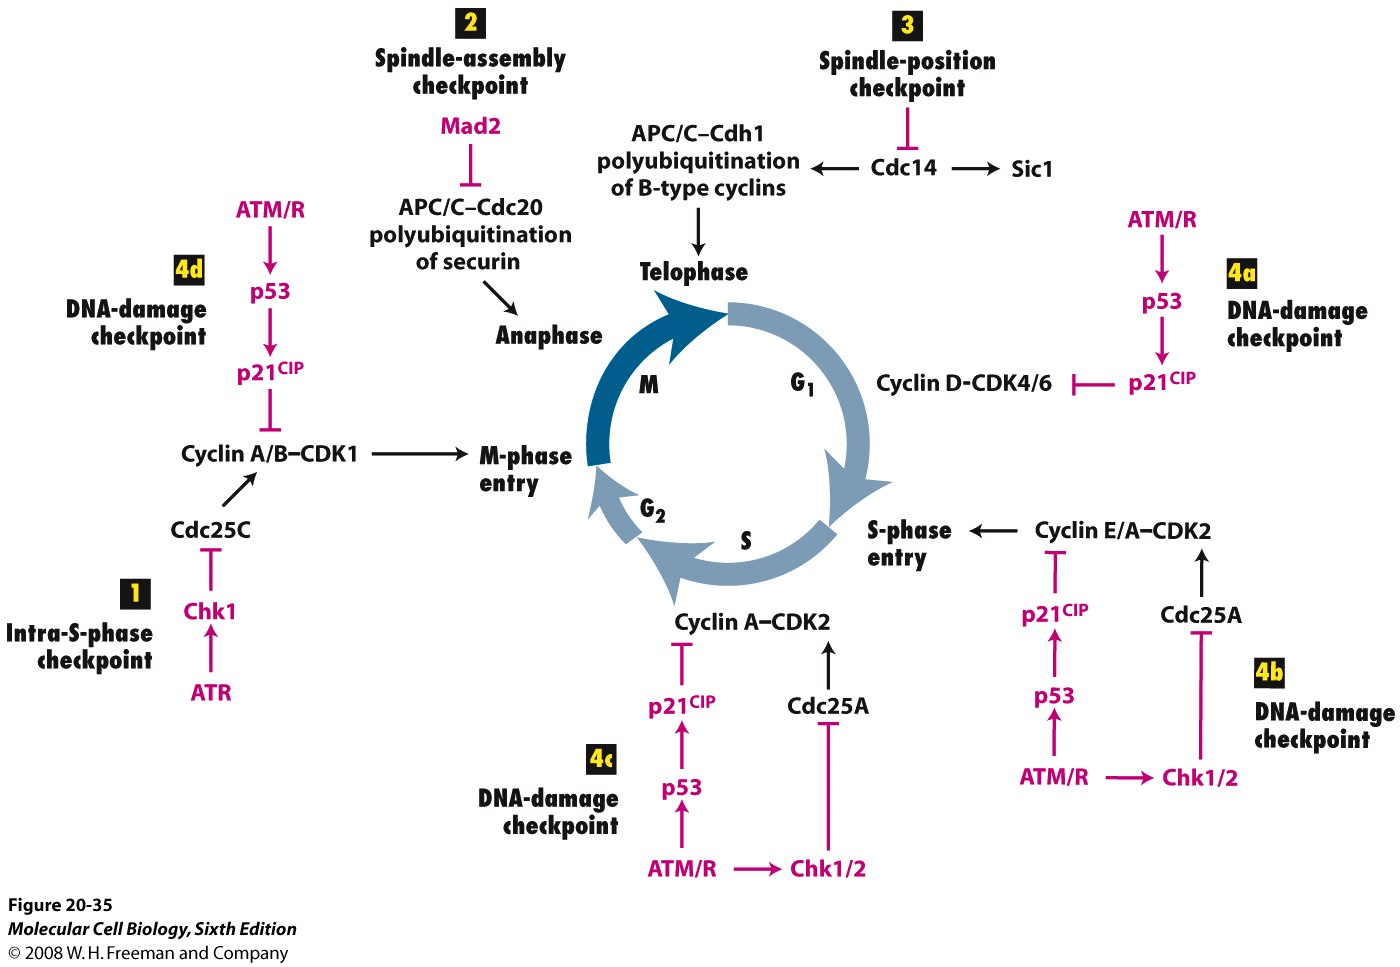
\includegraphics[width=\textwidth]{dnacheck}
\end{center}
\end{column}
\begin{column}{.4\textwidth}
\begin{block}{DNA kahjustused v\~oi replikatsioonikahvli arrest aktiveerivad kinaasid}
\begin{itemize}
  \item ATM (ataxia telangiectasia mutated) 
  \item ATR (ATM and Rad3-related)
\end{itemize}
\end{block}
\end{column}
\end{columns}
}
%%%%%%%%%%%%%%%%%%%%%%%
% DNA kontroll p53 s\~{o}ltuv ja p53-s\~{o}ltumatu
\subsection{p53}
\frame{\frametitle{DNA kvaliteedikontrolli mehhanismid: p53 s\~oltuv ja p53-s\~oltumatu rada}

\begin{center}
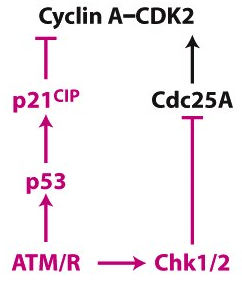
\includegraphics[width=.4\textwidth]{atrpathways}
\end{center}
}

%%%%%%%%%%%%%%%%%%%%%%
\subsection{tuumorsupressor}
\frame{\frametitle{p53 tuumorsupressor}
% \begin{block}{}
% \textbf{p53 on muteerunud keskmiselt 45\% kasvajates. Munasarja- v\"ahi puhul isegi 95\% juhtudel.}
% \end{block}
\begin{columns}
\begin{column}{.5\textwidth}
\begin{block}{p53 toimib mitme mehhanismi kaudu:}
\begin{itemize}
  \item Aktiveerib DNA reparatsiooni ens\"u\"ume, kui DNA on kahjustatud.
  \item Blokeerib rakuts\"ukli \"uleminekut G1/S kontrollpunktis.
  \item Suunab rakke apoptoosi.
\end{itemize}
\end{block}
\end{column}
\begin{column}{.5\textwidth}
\begin{center}
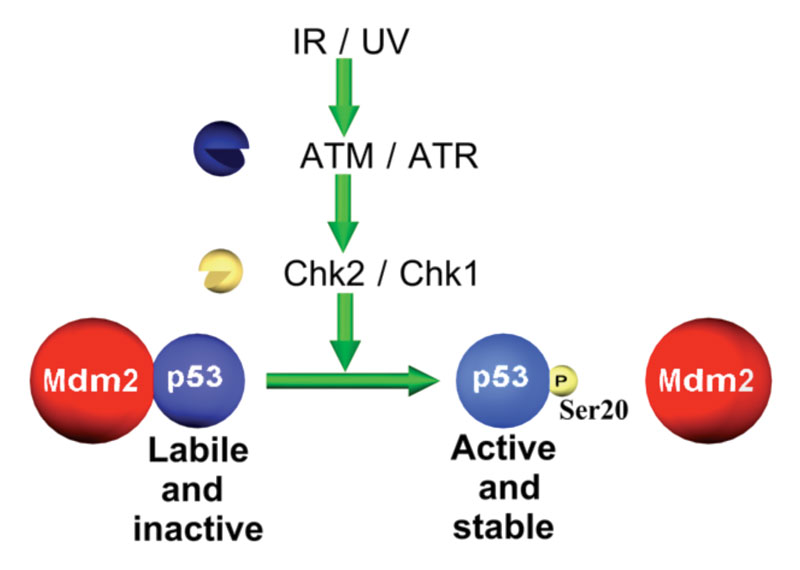
\includegraphics[width=\textwidth]{Haupt3color}
\end{center}
\end{column}
\end{columns}
}

%%%%%%%%%%%%%%%%%%%%%%
\subsection{tuumorsupressor2}
\frame{\frametitle{Mutantne p53}
\begin{block}{}
\textbf{p53 on muteerunud keskmiselt 45\% kasvajates. Munasarja- v\"ahi puhul isegi 95\% juhtudel.}
\end{block}

\begin{center}
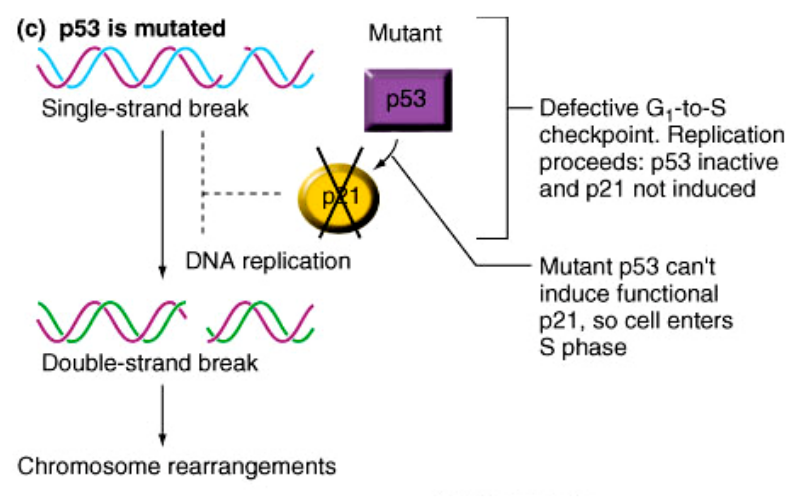
\includegraphics[width=.7\textwidth]{p53mutant}
\end{center}
}

%%%%%%%%%%%%%%%%%%%%%%
% % k\"a\"avi kontroll
% \subsection{k\"a\"av1}
% \frame{\frametitle{Kromatiidide lahknemine}
% 
% \begin{block}{\~Odekromatiide hoiavad koos kohesiinid}
% Kohesiinide lagundamist kontrollib APC$^{CDC20}$ ubikvitiin-ligaasi kompleks.
% \end{block}
% 
% \begin{center}
% 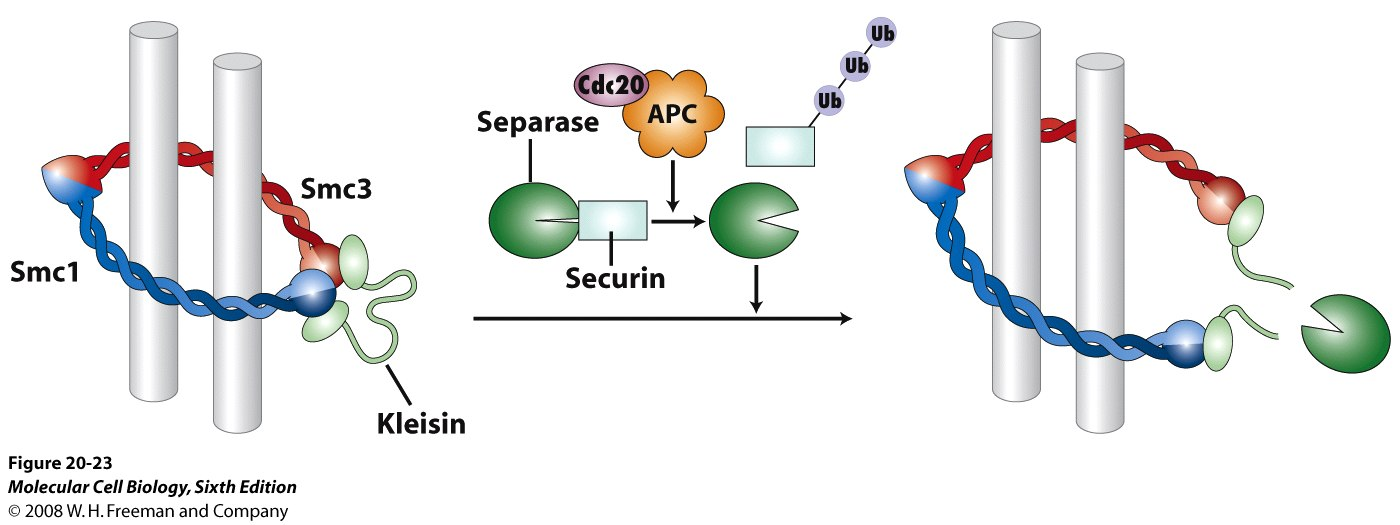
\includegraphics[width=\textwidth]{kohesiin}
% \end{center}
% }
% 
% % metafaasi kontroll -- kas k\"a\"aviniidid on kinnitunud kromosoomide kinetohoori
% \subsection{k\"a\"avi kontroll}
% \frame{\frametitle{Mitoosik\"a\"avi kontrollpunkt}
% 
% \begin{block}{Kas k\~oik kinetohoorid on seotud mitoosik\"a\"avi mikrotuubulitega?}
% \begin{itemize}
%   \item MAD (\emph{mitotic arrest deficient}) valk seostub vabadele kinetohooridele ja inhibeerib APC$^{CDC20}$ aktivatsiooni.
%   \item MAD seob ning blokeerib CDC20.
% \end{itemize}
% \end{block}

% \begin{center}
% 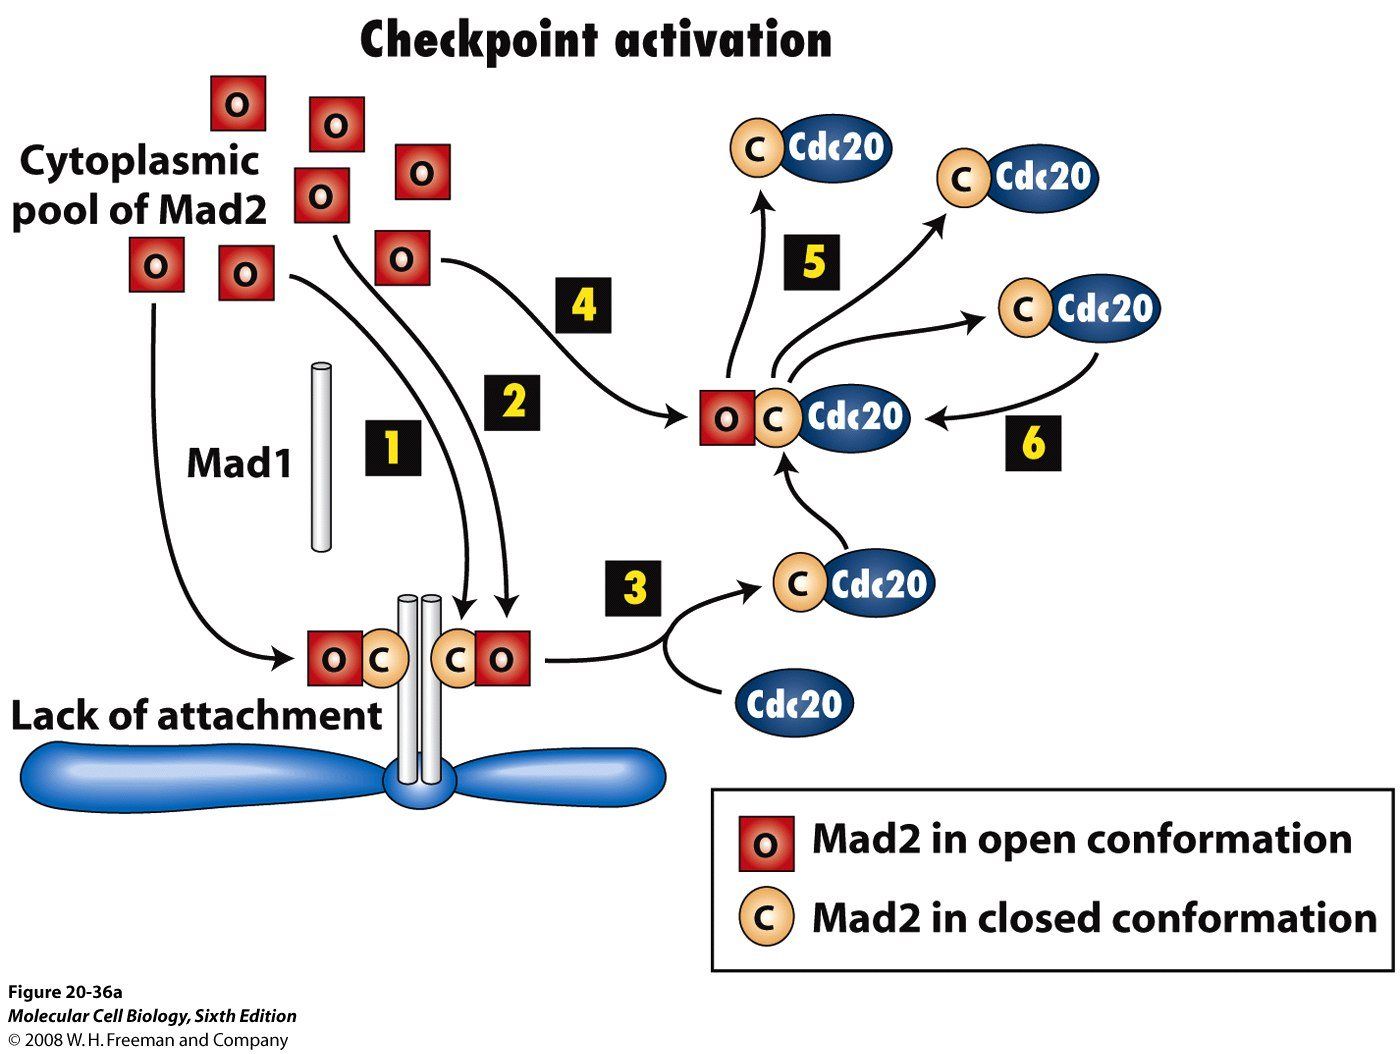
\includegraphics[width=.5\textwidth]{mad}
% \end{center}
% }
%%%%%%%%%%%%%%%%%%%%%%%%%
% %% TCGA mutations %%%%%%%
% \section{V\"ahk}
% \subsection{TCGA}
% \frame{\frametitle{Sagedasemad mutatsioonid kasvajates}
% \begin{center}
% 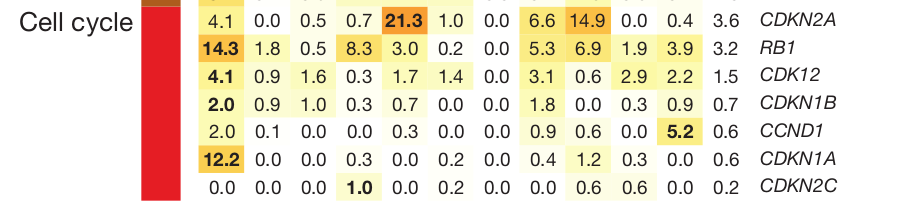
\includegraphics[width=.5\textwidth]{tcgacellcycle}
% 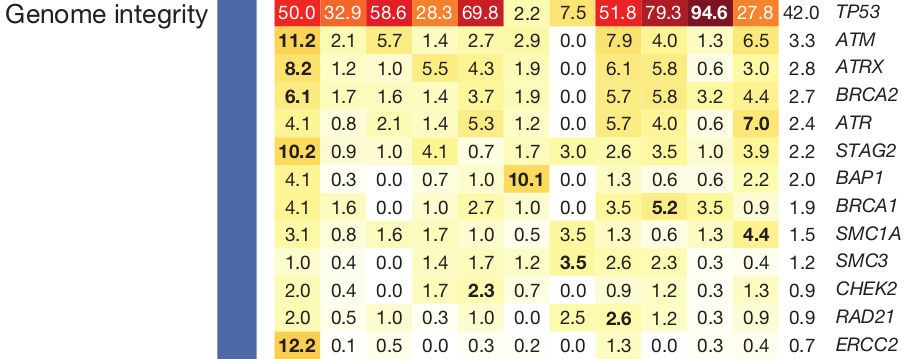
\includegraphics[width=.5\textwidth]{tcgagenomeint}
% \end{center}
% }


\end{document}
